%Prva naredba uvijek definira klasu dokumenta. Mi koristimo 'article'

\documentclass[a4paper,12pt,oneside]{article}




%***********************************************************************************
% Sada slijedi niz poziva Paketa funkcija cije ce se naredbe kasnije koristiti:
%***********************************************************************************

%Paket za upravljanje sa listama
\usepackage{enumitem}

% Paket za podesavanje brojeva stranica
\usepackage{scrlayer-scrpage}
	\ifoot[]{}
	\cfoot[]{}
	\ofoot[\pagemark]{\pagemark}
	\pagestyle{scrplain}


% Najcesce koristeni paketi za matematiku i formatiranje rada:
\usepackage{xurl}
\usepackage{url}
\usepackage{amsmath, amsthm}
\usepackage{mathtools}
\usepackage{latexsym,amsfonts,amssymb,amsbsy,graphics}
\usepackage{graphicx}
\usepackage[T1]{fontenc}
\usepackage[utf8]{inputenc}
\usepackage{mathptmx}
\usepackage{babel}
\babelprovide[import,main]{croatian} %Omogucava pisanje hrvatskih znakova
\usepackage[a4paper,left=25mm,right=20mm,top=25mm,bottom=25mm]{geometry}
\usepackage{microtype}
\usepackage{gensymb}
\usepackage{pdfpages}  %Omogucava importiranje stranica pdf fila u dokument
\usepackage{pdflscape} %Omogucava okretanje pojedine stranice landscape dok su ostale portrait


% Paket za postavke naslova i podnaslova
\usepackage{titlesec}
	\newcommand{\periodafter}[1]{#1.}
	\titleformat{\section}[hang]{\bf\large}{\thesection.}{5pt}{}{}
	\titleformat{\subsection}[hang]{\bf\large}{\thesubsection.}{3pt}{}{}
	\AtBeginDocument{%
		\let\sectionwithoutpagebreak\section
		\renewcommand{\section}{\clearpage\sectionwithoutpagebreak}%
	}

% Dva paketa za imenovanje slika i tablica
\usepackage{subcaption}
\usepackage[labelfont=bf,textfont=it,labelsep = colon]{caption}
	\captionsetup[figure]{name=SL.}
	\captionsetup[table]{name=Tab.}

% Paket sa bojama za formatiranje svega gdje se mjenja boja
\usepackage{xcolor}

% Paket za omogucavanje importiranja programskih kodova u tekst
\usepackage{listings}
	\lstset{
  		numbers=left,
  		numberstyle=\tiny,
  		columns=fullflexible,
  		breaklines=true,
  		postbreak=\mbox{\textcolor{red}{$\hookrightarrow$}\space},
  		xleftmargin=5.0ex
	}
	\renewcommand{\lstlistingname}{Primjer koda}% Listing -> Algorithm

% Paket za formatiranje Sadrzaja
\usepackage[dotinlabels]{titletoc}
	\dottedcontents{section}[5em]{\bfseries}{2em}{1pc}
	\dottedcontents{subsection}[7em]{}{2em}{1pc}



% Najbolji paket u svemiru za matematicko pisanje tekstova
\usepackage{physics}

% Paket za postavljanje linkova na koje se moze klikat u pdfu (prema formuli broj x- click odvede na to)
\usepackage{hyperref}
\hypersetup{
    colorlinks,
    linkcolor={red!50!black},
    citecolor={blue!50!black},
    urlcolor={blue!80!black}
}


% Postavke odlomaka

\setlength{\parindent}{0pt}
\setlength{\parskip}{0.6em}
\setlength{\headheight}{22pt}
\setlength{\footheight}{22pt}
\setlength{\footskip}{28pt}
\setlength{\emergencystretch}{2em}


%**************************************************************************************************************
% Prostor za tvoje pakete je ovdje:
%**************************************************************************************************************

\usepackage{booktabs}
\usepackage{array}
\usepackage{longtable}
\usepackage{float}


%**************************************************************************************************************





%Kraj preamble naredbi, krece se sa pisanjem dokumenta
%**************************************************************************************************************


\begin{document}

%**************************************************************************************************************
% Postavke za numeriranje, prorede i ostalo
%**************************************************************************************************************

\setcounter{MaxMatrixCols}{20}                          %Postavka da matrica moze imati vise od 10 stupaca
\renewcommand{\baselinestretch}{1.5}                    %postavke za prored 1.5%
\makeatletter
\@addtoreset{figure}{section}
\@addtoreset{table}{section}
\@addtoreset{equation}{section}
\makeatother
\renewcommand{\thefigure}{\thesection.\arabic{figure}}  %postavke za imenovanje slika po poglavljima%
\renewcommand{\thetable}{\thesection.\arabic{table}}   %postavke za imenovanje tablica po poglavljima%
\renewcommand{\theequation}{\thesection-\arabic{equation}} %postavke za brojanje jednadzbi po poglavljima%
\renewcommand{\refname}{LITERATURA}						% Uppercase Literatura
\pagenumbering{gobble}
\hypersetup{pageanchor=false}

%**************************************************************************************************************




%**************************************************************************************************************
% NASLOVNA STRANICA
%**************************************************************************************************************

\begin{titlepage}

\begin{center}
{\bfseries\fontsize{14}{16}\selectfont SVEUČILIŠTE JOSIPA JURJA STROSSMAYERA U OSIJEKU}\\
{\bfseries\fontsize{14}{16}\selectfont FAKULTET ELEKTROTEHNIKE, RAČUNARSTVA I INFORMACIJSKIH}\\
{\bfseries\fontsize{14}{16}\selectfont TEHNOLOGIJA OSIJEK}\\
\bigskip

\vspace*{2cm}
{\bfseries\fontsize{14}{16}\selectfont Sveučilišni diplomski studij Računarstvo}\\
{\bfseries\fontsize{14}{16}\selectfont DRB -- Umjetna inteligencija i robotika}

\vspace*{5cm}

{\bfseries\fontsize{18}{22}\selectfont AUTOMATSKA SEGMENTACIJA SUSPEKTNIH LEZIJA PROSTATE IZ MULTIMODALNIH MR SNIMKI PRIMJENOM DUBOKOG UČENJA}

\vspace*{1cm}
{\bfseries\fontsize{14}{16}\selectfont Diplomski rad}\\
\vspace*{3cm}
{\bfseries\fontsize{16}{18}\selectfont Ramal Salha}\\
\vfill
{\bfseries\fontsize{14}{16}\selectfont Osijek, 2026.}
\end{center}

\end{titlepage}



%**************************************************************************************************************
% OBRASCI I FORMULARI
%**************************************************************************************************************

% Obrazac D1 i izjavu o izvornosti rada ne treba umetati u radnu verziju ako ih sustav MAK automatski dodaje u konačnu verziju.


%\newpage
%\includepdf{D1_obrazac.pdf}
%\newpage
%\includepdf{Originalnost.pdf}
%\newpage




%**************************************************************************************************************
% TABLE OF CONTENTS
%**************************************************************************************************************

{
	\hypersetup{linkcolor=black}
	\tableofcontents
}
%**************************************************************************************************************



\newpage
\pagenumbering{arabic}
\setcounter{page}{1}
\hypersetup{pageanchor=true}

\section{UVOD}

Rak prostate jedna je od bolesti kod kojih magnetska rezonancija ima važnu ulogu u dijagnostičkom postupku i planiranju daljnje obrade. U višemodalnom MR pregledu prostate najčešće se koriste anatomske T2-mjerene snimke te funkcionalne sekvence kao što su ADC i difuzijski ponderirane snimke visokih b-vrijednosti. Ručno označavanje suspektnih lezija na takvim volumenima zahtijeva stručno znanje, vrijeme i dosljednu interpretaciju više slikovnih modaliteta. Zbog toga je automatska segmentacija lezija prikladan problem za primjenu dubokog učenja (engl. \textit{deep learning}), ali je istodobno zahtjevna zbog malog volumena lezija, neravnoteže između pozitivnih i negativnih voksela te razlika između skupova podataka.

Tema ovog rada je razvoj i evaluacija postupka za automatsku segmentaciju suspektnih lezija prostate iz multimodalnih MR snimki. U sklopu rada razvijen je programski sustav za učitavanje i predobradu podataka, nadzirano treniranje segmentacijskih modela, samonadzirano predtreniranje (engl. \textit{self-supervised pretraining}) enkodera (engl. \textit{encoder}), evaluaciju spremljenih modela, vizualizaciju rezultata i analizu modela jednostavnim metodama objašnjivosti. Glavni ulazni modaliteti u provedenim eksperimentima su T2w, ADC i HBV, a cilj segmentacije je binarna maska suspektne lezije.

U radu se ne pretpostavlja klinička spremnost razvijenog sustava. Eksperimenti se promatraju kao istraživačka usporedba nekoliko arhitektura i konfiguracija na ograničenim testnim skupovima. Posebno se analiziraju rezultati na fiksnom PI-CAI testnom skupu od 10 slučajeva i dodatnom vanjskom skupu od 19 slučajeva iz skupa Prostate158, kako bi se jasnije prikazalo ponašanje modela unutar početnog skupa podataka i izvan njega.

\subsection{Zadatak rada}

% TODO: Dodati službeni tekst zadatka diplomskog rada iz FERIT/MAK sustava.

Zadatak rada obuhvaća pripremu višemodalnih MR podataka, implementaciju i usporedbu više modela za segmentaciju lezija prostate, definiranje evaluacijskih metrika, provođenje eksperimenata, prikaz kvalitativnih rezultata i analizu ponašanja modela metodama objašnjivosti.

\subsection{Struktura rada}

U drugom poglavlju prikazana je klinička i slikovna pozadina zadatka te pregled povezanih metoda i skupova podataka. Treće poglavlje opisuje podatke i predobradu. U četvrtom poglavlju prikazana je arhitektura programskog sustava i veza između glavnih programskih modula. Peto poglavlje opisuje eksperimentalni postav i metrike. Šesto poglavlje donosi rezultate i raspravu, a sedmo poglavlje prikazuje korištene metode objašnjivosti modela. Zaključno poglavlje sažima provedeni rad, ograničenja i moguće smjerove nastavka.

\section{PREGLED PODRUČJA TEME}

\subsection{Rak prostate i suspektne lezije}

Rak prostate u radiološkom se postupku ne promatra samo kao pitanje prisutnosti ili odsutnosti bolesti, nego i kroz procjenu kliničke značajnosti nalaza. U skupovima podataka korištenima u ovom radu cilj segmentacije vezan je uz suspektne lezije, odnosno područja na MR snimkama koja su označena kao mogući klinički značajan karcinom prostate. U PI-CAI skupu pozitivni slučajevi definirani su u kontekstu klinički značajnog karcinoma prostate, pri čemu su oznake lezija dostupne kao prostorne maske \cite{picai_dataset,picai_labels}. U ovom radu te se oznake ne koriste za procjenu stupnja bolesti, nego isključivo kao binarni cilj segmentacije.

Takva formulacija zadatka razlikuje se od cjelovitog dijagnostičkog postupka. Segmentacijski model računa prostornu masku na temelju slikovnih podataka i ne uključuje sve informacije koje se u kliničkoj praksi mogu uzeti u obzir, primjerice laboratorijske nalaze, anamnezu, prethodne biopsije ili radiološki izvještaj. Zbog toga se razvijeni sustav u radu tumači kao istraživački postupak za računalnu segmentaciju lezija, a ne kao samostalan dijagnostički sustav.

% TODO: Dodati provjerenu medicinsku referencu za epidemiološki i klinički opis raka prostate ako se ovo poglavlje bude dodatno širilo.

\subsection{Modaliteti MR snimanja prostate}

Višemodalni MR pregled prostate spaja anatomske i funkcionalne informacije. T2-mjerena snimka prikazuje građu prostate i okolnih tkiva te daje referentni anatomski kontekst. Difuzijske snimke i karte prividnog difuzijskog koeficijenta opisuju ograničenje difuzije vode u tkivu, pa mogu naglasiti područja koja se na T2w snimci ne vide jednako jasno. U ovom radu ulaz modela najčešće čine T2w, ADC i HBV kanal, pri čemu HBV označava difuzijski ponderiranu snimku visoke b-vrijednosti.

Korištenje više modaliteta ne znači da je svaki modalitet jednako informativan u svakom slučaju. T2w kanal u implementaciji ima i praktičnu ulogu referentnog prostora: ADC i HBV volumen registriraju se i ponovno uzorkuju u prostornu mrežu T2w snimke. Time se omogućuje slaganje modaliteta u isti ulazni tenzor, ali se ne uklanja potpuno mogućnost lokalnih neporavnanja između sekvenci. Ta je mogućnost važna pri tumačenju pogrešaka jer segmentacijski model očekuje da isti prostorni položaj kroz kanale opisuje isto anatomsko područje.

\subsection{PI-RADS i opseg rada}

PI-RADS je sustav za strukturirano tumačenje MR pregleda prostate i procjenu sumnje na klinički značajan karcinom prostate \cite{pirads_v21}. U kontekstu ovog rada PI-RADS je važan zato što objašnjava zašto se T2w, ADC i difuzijske snimke promatraju zajedno te zašto se zadatak ne svodi na obradu jednog slikovnog kanala. Ipak, implementirani sustav ne dodjeljuje PI-RADS ocjene i ne pokušava reproducirati kompletan radiološki postupak.

Ograničenje je posebno važno naglasiti jer segmentacijska maska nije jednaka kliničkoj odluci. Model može proizvesti prostorno uvjerljivu masku, ali to samo po sebi ne dokazuje kliničku značajnost nalaza. U radu se zato rezultati vrednuju metrikama segmentacije i kvalitativnim prikazima, dok se tvrdnje o dijagnostičkoj upotrebljivosti ne iznose.

\subsection{Duboko učenje za segmentaciju medicinskih slika}

Segmentacija medicinskih slika dubokim učenjem najčešće se formulira kao učenje preslikavanja iz slikovnog volumena u masku anatomskog ili patološkog područja. Kod lezija prostate problem je dodatno otežan time što lezije mogu zauzimati mali dio volumena, mogu biti slabo vidljive na pojedinačnom modalitetu i često zahtijevaju zajedničko tumačenje anatomskih i funkcionalnih informacija.

Polazna arhitektura za mnoge medicinske segmentacijske sustave je U-Net, koji kombinira kontrakcijski put za izdvajanje konteksta i ekspanzijski put za vraćanje prostorne rezolucije, uz preskočne veze (engl. \textit{skip connections}) između odgovarajućih razina \cite{unet}. Za volumetrijske medicinske podatke razvijena je 3D varijanta U-Neta, u kojoj se 2D operacije zamjenjuju 3D konvolucijama i tako omogućuju izravnu obradu volumena \cite{unet3d}. Takav pristup prirodno odgovara MR podacima jer lezija nije izolirana na jednom presjeku, nego se prostire kroz više susjednih aksijalnih slojeva.

Attention U-Net nadograđuje U-Net pažnjom (engl. \textit{attention}) na preskočnim vezama \cite{attention_unet}. Umjesto da se sve enkoderske značajke bezuvjetno prenesu u dekoder (engl. \textit{decoder}), pažnja ih prostorno ponderira prema dekoderskom signalu. U zadatku segmentacije lezija prostate to je zanimljivo jer preskočne veze čuvaju detaljnu prostornu informaciju, ali istodobno mogu prenijeti mnogo pozadinskog signala. U ovom radu Attention U-Net 3D koristi se kao glavna konvolucijska polazna arhitektura i uspoređuje se s novijim pristupima.

Važan smjer u medicinskoj segmentaciji predstavlja nnU-Net, okvir koji ne uvodi novu osnovnu arhitekturu, nego sustavno prilagođava predobradu, veličine isječaka, konfiguraciju U-Neta, treniranje i inferenciju (engl. \textit{inference}) svojstvima pojedinog skupa podataka \cite{nnunet}. U ovom radu nije implementiran puni nnU-Net postupak, ali su neke praktične ideje slične: odabir volumetrijskih isječaka prema memorijskim ograničenjima, korištenje kliznog prozora (engl. \textit{sliding window}) u validaciji, normalizacija intenziteta i čuvanje konfiguracije eksperimenta uz rezultate.

U ovom radu PI-CAI se koristi kao glavni skup za nadziranu segmentaciju suspektnih lezija prostate. Skup je javno dostupan i sadrži 1500 slučajeva s višemodalnim MR snimkama i oznakama lezija \cite{picai_dataset}. Kao dodatni vanjski skup koristi se Prostate158, koji sadrži ekspertno označene 3T MR snimke prostate i popratne anotacije \cite{prostate158_main,prostate158_dib}. Prostate158 služi za dodatnu evaluaciju, a njegovi neoznačeni volumeni korišteni su i u samonadziranom predtreniranju.

Uspoređene su tri obitelji modela. Attention U-Net 3D korišten je kao konvolucijska polazna arhitektura s pažnjom na preskočnim vezama. Deconver je uključen kao novija segmentacijska arhitektura koja koristi dekonvolucijsko miješanje značajki \cite{deconver}. FCT je uključen kao transformatorski nadahnuta usporedna arhitektura za medicinsku segmentaciju \cite{fct}, uz motivaciju iz konvolucijskih vidnih transformera \cite{cvt}. Budući da je FCT izvorno razvijen za 2D segmentaciju, prilagođen je volumetrijskom sučelju obradom aksijalnih presjeka i ponovnim slaganjem predikcija u 3D volumen.

U kasnijoj fazi projekta dodana je i podrška za DynUNet i SwinUNETR. DynUNet se može promatrati kao praktična, konfigurabilna varijanta U-Net pristupa u kojoj se dubina, koraci promjene rezolucije, veličine jezgri i broj značajki mogu prilagoditi svojstvima volumetrijskog skupa podataka. SwinUNETR pripada skupini transformatorski zasnovanih volumetrijskih segmentacijskih modela: ulaz se obrađuje kroz hijerarhijske transformatorske blokove s lokalnim prozorima pažnje, a dekoderski dio ponovno gradi segmentacijsku masku na punoj prostornoj rezoluciji. U ovom radu su te dvije arhitekture važne kao dodatni smjer usporedbe, ali njihovi rezultati još nisu uključeni u prikazane tablice.

% TODO: Dodati provjerene reference za DynUNet/MONAI i SwinUNETR prije konačne verzije teorijskog pregleda.

Razlika između ovog rada i navedenih općih arhitektura nije u predlaganju potpuno nove mreže, nego u izgradnji cjelovitog eksperimentalnog postupka za jedan konkretan problem: višemodalnu segmentaciju suspektnih lezija prostate, usporedbu nekoliko arhitektura pod istim evaluacijskim uvjetima, dodatnu provjeru na Prostate158 skupu i kvalitativnu analizu ponašanja modela. U tom smislu rad se oslanja na postojeće metode, ali ih povezuje s vlastitim tijekom učitavanja, predobrade, treniranja, evaluacije i vizualizacije.

\section{SKUP PODATAKA I PREDOBRADA}

\subsection{Skup PI-CAI}

Glavni skup podataka u radu je javni PI-CAI (\textit{Prostate Imaging: Cancer AI}) skup za razvoj i evaluaciju metoda za računalnu analizu magnetske rezonancije prostate \cite{picai_dataset}. Skup je nastao u okviru izazova PI-CAI, čiji je cilj usporedba algoritama umjetne inteligencije i radiološke interpretacije pri detekciji klinički značajnog karcinoma prostate na biparametrijskim MR snimkama. U tom kontekstu PI-CAI nije samo zbirka slikovnih volumena, nego i standardiziran istraživački okvir s definiranim slučajevima, oznakama lezija i metapodacima potrebnima za razvoj sustava za detekciju i segmentaciju suspektnih područja.

Javni dio skupa sadrži 1500 anonimiziranih MR pregleda prostate iz 1476 bolesnika, snimljenih između 2012. i 2021. godine u tri nizozemska centra. Podaci obuhvaćaju snimanja s više uređaja i lokacija, što je važno jer modeli ne uče samo morfologiju lezija, nego su izloženi i razlikama u protokolima, rezolucijama, kontrastu i šumu između akvizicija. Prema opisu skupa, 425 slučajeva označeno je kao klinički značajan karcinom prostate, dok 1075 slučajeva pripada benignim nalazima ili indolentnom karcinomu prostate. Takav odnos pozitivnih i negativnih slučajeva stvara izraženu neravnotežu podataka, osobito kada se problem promatra na razini voksela jer lezije zauzimaju malen dio volumena.

Za svaki slučaj dostupne su najmanje tri aksijalne sekvence: T2-mjerena snimka (T2w), karta prividnog difuzijskog koeficijenta (ADC) i difuzijski ponderirana snimka visoke b-vrijednosti (HBV). T2w prikazuje anatomsku građu prostate i okolnih struktura, dok ADC i HBV nose funkcionalne informacije povezane s difuzijom vode u tkivu. U izvornom skupu mogu postojati i sagitalne ili koronarne T2w snimke, ali se one u ovom radu ne koriste. Programsko rješenje zato očekuje i obrađuje tri aksijalna modaliteta, pri čemu T2w služi kao referentni prostor za registraciju ostalih modaliteta.

Oznake povezane sa skupom PI-CAI dostupne su odvojeno od slikovnih datoteka, preko repozitorija s anotacijama \cite{picai_labels}. One uključuju razgraničenja klinički značajnih lezija, zapise o ishodu slučaja i dodatne resurse kao što su automatski dobivene maske cijele prostate. U ovom radu oznake lezija ne koriste se kao višeklasni problem određivanja stupnja bolesti, nego se svaka nenulta vrijednost u oznaci prevodi u vrijednost 1. Time se zadatak svodi na binarnu segmentaciju: model za svaki voksel procjenjuje pripada li suspektnoj leziji ili pozadini. Sažetak korištenih podataka prikazan je u tablici~\ref{tab:dataset_summary}.

\begin{table}[H]
\centering
\caption{Sažetak glavnog nadziranog skupa podataka. \label{tab:dataset_summary}}
\begin{tabular}{>{\raggedright\arraybackslash}p{0.42\textwidth} >{\raggedright\arraybackslash}p{0.42\textwidth}}
\toprule
Svojstvo & Vrijednost \\
\midrule
Naziv skupa & PI-CAI \\
Vrsta snimanja & Biparametrijska MR snimka prostate \\
Ukupan broj pregleda & 1500 \\
Broj bolesnika & 1476 \\
Razdoblje akvizicije & 2012.--2021. \\
Izvori podataka & Tri klinička centra u Nizozemskoj \\
Pozitivni slučajevi & 425 slučajeva s klinički značajnim karcinomom prostate \\
Negativni slučajevi & 1075 benignih ili indolentnih slučajeva \\
Obvezni modaliteti u skupu & Aksijalni T2w, ADC i HBV \\
Modaliteti korišteni u radu & T2w, ADC i HBV \\
Korištena oznaka & Binarna maska lezije dobivena iz nenultih vrijednosti anotacije \\
Zadatak u ovom radu & Binarna segmentacija suspektne lezije \\
\bottomrule
\end{tabular}
\end{table}

Slikovne datoteke u PI-CAI skupu organizirane su prema identifikatoru bolesnika i pregleda, a nazivi datoteka označavaju pripadajući modalitet. U implementaciji se slučaj prepoznaje prema zajedničkom identifikatoru, nakon čega se povezuju T2w, ADC i HBV volumen te pripadajuća datoteka oznake. Takva organizacija omogućuje da se nad istim slučajem dosljedno provedu registracija, ponovno uzorkovanje i slaganje modaliteta u ulazni tenzor modela. Budući da se negativni slučajevi uče s praznom maskom lezije, oni su važni za smanjenje lažno pozitivnih predikcija, ali istodobno zahtijevaju pažljivo definiranje funkcije gubitka i evaluacijskih metrika.

Za usporedivu evaluaciju u ovom radu izdvojen je fiksni PI-CAI testni skup od 10 slučajeva, od čega je 5 pozitivnih i 5 negativnih. Ti slučajevi nisu korišteni pri treniranju ni validaciji. Preostali PI-CAI slučajevi korišteni su za učenje i validaciju modela.

\subsection{Skup Prostate158}

Prostate158 se koristi kao dodatni vanjski skup za provjeru ponašanja modela izvan glavnog PI-CAI skupa \cite{prostate158_main,prostate158_dib}. Skup sadrži 3T MR snimke prostate s pripadajućim anotacijama, uključujući tumorske oznake i oznake anatomskih područja prostate. U ovom radu Prostate158 ima dvije uloge. Prva je dodatna evaluacija modela treniranih u glavnom PI-CAI postupku, a druga je korištenje neoznačenih volumena u samonadziranom predtreniranju.

Za evaluaciju je korišteno 19 Prostate158 testnih slučajeva. Budući da je riječ o drugom izvoru podataka, razlike u akviziciji, organizaciji datoteka, oznakama i intenzitetima mogu utjecati na izlaz modela. Zato se rezultati na Prostate158 skupu ne tumače kao potpuna vanjska klinička validacija, nego kao ograničena provjera prijenosa između skupova podataka. U implementaciji se Prostate158 slučajevi čitaju iz pripadajućih CSV datoteka, pri čemu se T2 kanal preslikava u T2w ulaz, ADC u ADC ulaz, a DWI se koristi kao zamjena za HBV kanal.

\subsection{Volumetrijski format podataka}

Ulazni podaci nisu pojedinačne 2D slike, nego 3D volumeni. Svaki volumen može se promatrati kao niz aksijalnih presjeka s pripadajućim informacijama o razmaku između voksela, orijentaciji i fizičkom položaju u prostoru. Te informacije su bitne jer se T2w, ADC, HBV i oznaka lezije moraju nalaziti u istom prostornom sustavu prije slaganja u ulaz modela. U PI-CAI skupu slikovni volumeni učitavaju se iz medicinskih slikovnih datoteka u MHA formatu, dok su oznake lezija pohranjene kao NIfTI datoteke s nastavkom \texttt{.nii.gz}. Prostate158 u implementaciji koristi NIfTI volumene za slikovne kanale i oznake.

Nakon učitavanja svaki se modalitet pretvara u numerički volumen oblika $(D, H, W)$, gdje $D$ označava broj aksijalnih presjeka, a $H$ i $W$ prostorne dimenzije presjeka. Modaliteti se zatim slažu po kanalskoj dimenziji, pa model prima tenzor oblika $(C, D, H, W)$ za jedan slučaj, odnosno $(B, C, D, H, W)$ tijekom treniranja. Takav zapis omogućuje da 3D konvolucijski modeli obrađuju prostorni kontekst kroz više presjeka, dok FCT u ovom projektu isti volumen interno rastavlja na aksijalne 2D presjeke.

Tok pripreme jednog slučaja prikazan je na slici~\ref{fig:data_flow}. Slika naglašava da se registracija i ponovno uzorkovanje provode prije slaganja kanala, jer bi u suprotnom isti indeks voksela mogao označavati različite fizičke položaje u različitim modalitetima.

\begin{figure}[H]
\centering
\fbox{%
\begin{minipage}{0.90\textwidth}
\centering
\begin{tabular}{>{\centering\arraybackslash}p{0.84\textwidth}}
T2w volumen, ADC volumen, HBV/DWI volumen i oznaka lezije \\
$\downarrow$ \\
učitavanje metapodataka, orijentacije i razmaka voksela \\
$\downarrow$ \\
registracija ADC i HBV/DWI volumena u T2w prostor \\
$\downarrow$ \\
ponovno uzorkovanje na ciljnu rezoluciju i binarizacija oznake \\
$\downarrow$ \\
z-vrijednosna normalizacija intenziteta po modalitetu \\
$\downarrow$ \\
slaganje kanala u tenzor $(C, D, H, W)$ i uzorkovanje 3D isječaka
\end{tabular}
\end{minipage}}
\caption{Tok pripreme višemodalnog volumena prije ulaza u segmentacijski model. \label{fig:data_flow}}
\end{figure}

Prikazani tok vrijedi za osnovnu segmentaciju lezija bez dodatnog ograničavanja prostora obrade. U repozitoriju su implementirani i ROI postupci te lokalizatori prostate, ali stariji stabilni skup rezultata prikazan u ovom radu ne oslanja se na njihove artefakte. Zbog toga se pri tumačenju rezultata mora posebno navesti koja je konfiguracija, ako je primjenjivo, koristila ROI izrezivanje ili lokalizator prostate.

\subsection{Učitavanje i predobrada}

U projektu je napravljen postupak koji iz dostupnih datoteka za svaki slučaj povezuje T2w, ADC i HBV volumen s odgovarajućom oznakom lezije. PI-CAI podaci učitavaju se iz izvorne strukture skupa podataka, dok se slučajevi iz Prostate158 skupa odabiru prema pripadajućim popisima slučajeva. Oznake lezija koriste se kao binarne maske, pri čemu se zadatak svodi na razlikovanje voksela lezije od pozadine.

Predobrada uključuje registraciju ADC i HBV volumena u prostor referentne T2w snimke, ponovno uzorkovanje na ciljnu prostornu rezoluciju, pretvorbu u tenzore oblika $(C, D, H, W)$ i normalizaciju intenziteta. Ciljna rezolucija u konfiguracijama prikazanih pokretanja iznosi $(3.0, 0.5, 0.5)$~mm po osima $(z, y, x)$. Za slikovne modalitete koristi se linearna interpolacija, dok se oznake ponovno uzorkuju interpolacijom najbližeg susjeda kako bi vrijednosti maske ostale diskretne. Normalizacija je z-vrijednosna i računa se primarno nad nenultim vokselima kako bi se smanjio utjecaj pozadine. Kod Prostate158 podataka difuzijski ponderirana snimka koristi se kao zamjena za HBV kanal, uz predobradu koja uključuje ograničavanje intenziteta percentilima i logaritamsku kompresiju dinamičkog raspona.

Kao dodatni oblik predobrade sustav podržava ograničavanje ulaznog volumena na područje interesa, odnosno ROI. Taj postupak nije jednak uzorkovanju 3D isječaka tijekom treniranja. ROI izrezivanje najprije smanjuje cijeli resamplirani volumen na područje oko prostate, a tek se nakon toga iz tako ograničenog volumena mogu uzorkovati manji isječci za učenje modela.

Granice izreza određuju se iz binarne ROI maske. Maska se najprije binarizira, nakon čega se pronalazi najmanji okvir koji obuhvaća sve pozitivne voksele. Na taj se okvir dodaje zadana margina izražena u milimetrima, koja se prema razmaku voksela pretvara u broj voksela po osima $(z, y, x)$. Zatim se provjerava minimalna dopuštena veličina izreza kako bi ulaz ostao prikladan za model i za kasnije uzorkovanje isječaka. Ako proširene granice izlaze izvan volumena, ograničavaju se na stvarne dimenzije slike. U slučaju prazne ROI maske može se koristiti povratni postupak u kojem se zadržava puni volumen.

ROI maska može potjecati iz dostupne oznake prostate ili iz prethodno istreniranog lokalizacijskog modela. Kada se segmentacija računa samo nad izrezanim područjem, izlaz se pri validaciji i evaluaciji može vratiti u koordinatni sustav punog resampliranog volumena tako da se predikcija upiše na mjesto izreza, a ostatak volumena ostane pozadina. Time se omogućuje usporedba s referentnom maskom u istoj prostornoj mreži.

U implementaciji se razlikuju tri načina rada ROI postupka. Prvi način ne koristi izrezivanje i zadržava puni resamplirani volumen. Drugi način koristi dostupnu masku prostate kao prostorno ograničenje, što je primjenjivo samo kada je takva oznaka dostupna i kada se ne koristi informacija koja ne bi bila poznata u stvarnoj inferenciji. Treći način koristi predviđenu masku prostate iz zasebnog lokalizacijskog modela. U tom se slučaju lokalizator najprije pokreće nad cijelim volumenom, njegova se predikcija binarizira i po potrebi svodi na najveću povezanu komponentu, a zatim se iz nje računaju granice izreza za segmentacijski model. Takav postupak omogućuje ispitivanje može li prostorno ograničavanje smanjiti lažno pozitivne predikcije, ali se u ovom radu ne miješa s glavnom usporedbom modela jer za njega nisu prikazani jednako stabilni rezultati kao za osnovni tijek segmentacije.

% TODO: Ako se ROI/lokalizator uključi u završne rezultate, dodati zasebnu tablicu koja uspoređuje puni volumen, ROI iz oznake prostate i ROI iz predviđene maske prostate na istom testnom skupu.

Učitavanje podržava PI-CAI organizaciju u ravnom direktoriju i ugniježđenu organizaciju po bolesniku i pregledu. T2w datoteka obvezna je u svakom slučaju jer služi kao referentna mreža za registraciju i ponovno uzorkovanje. ADC i HBV provjeravaju se samo ako su uključeni u konfiguraciji aktivnih modaliteta. Ako oznaka ne postoji, slučaj se može koristiti u postupcima koji ne zahtijevaju masku, primjerice u samonadziranom predtreniranju, dok nadzirano treniranje segmentacije očekuje pripadajuću oznaku.

Tijekom treniranja se iz volumena ne uzimaju samo slučajni isječci iz cijelog prostora, nego se koristi uzorkovanje koje povećava vjerojatnost da isječak sadrži leziju. U konfiguracijama se parametar \texttt{pos\_fraction} koristi za omjer pozitivnih i negativnih isječaka, a u prikazanim pokretanjima najčešće iznosi 0,75 ili 0,85. Osim toga, slučajevi u skupu za treniranje ponderiraju se prema prisutnosti lezije kako bi pozitivni i negativni slučajevi bili zastupljeniji u uravnoteženijem omjeru nego što bi to bilo kod potpuno slučajnog odabira. Takva dva koraka ne uklanjaju neravnotežu voksela, ali smanjuju mogućnost da model tijekom učenja pretežno vidi pozadinu.

Nad isječcima se primjenjuju geometrijske i intenzitetske augmentacije (engl. \textit{augmentations}). Geometrijske augmentacije uključuju zrcaljenja, rotacije, afine transformacije i elastične deformacije, pri čemu se iste prostorne transformacije primjenjuju na sliku i masku. Intenzitetske augmentacije uključuju šum, zaglađivanje, skaliranje i pomak intenziteta, promjenu kontrasta, simulaciju nehomogenosti polja i Gibbsov šum. Validacijski skup ne prolazi takve augmentacije, nego se puni resamplirani volumen predaje modelu kroz klizni prozor.

\section{ARHITEKTURA I IMPLEMENTACIJA SUSTAVA}

Programski sustav osmišljen je tako da se pojedini eksperiment može opisati konfiguracijom, a zatim ponovljivo pokrenuti kroz isti slijed koraka: priprema podataka, izgradnja modela, treniranje, validacija, spremanje najboljeg modela i naknadna evaluacija. Takva organizacija omogućila je usporedbu više arhitektura i postavki bez ručnog mijenjanja osnovnog tijeka izvođenja. Za svako pokretanje čuvaju se konfiguracija, metapodaci, zapisi učenja i spremljene kontrolne točke modela, što olakšava kasniju analizu rezultata.

\subsection{Nadzirano treniranje}

Nadzirano treniranje započinje učitavanjem konfiguracije eksperimenta i pripremom skupova za treniranje i validaciju. Za svaki odabrani model postavljaju se funkcija gubitka, optimizator i raspored promjene stope učenja. Tijekom učenja model ne obrađuje uvijek cijeli volumen odjednom, nego se koriste slučajno odabrani 3D isječci. Time se smanjuje memorijsko opterećenje i povećava raznolikost primjera koje model vidi tijekom jedne epohe. U validaciji se predikcija računa nad cijelim volumenom primjenom kliznog prozora, pa se dobiva izlaz koji je usporediv sa stvarnom 3D maskom lezije. Najbolji model odabire se prema kompozitnom validacijskom rezultatu koji može uključivati Dice, osjetljivost i HD95, ovisno o konfiguraciji.

Funkcija gubitka u stabilnim pokretanjima najčešće je Tversky+BCE. Tverskyjev dio omogućuje odvojeno ponderiranje lažno pozitivnih i lažno negativnih voksela, dok BCE dio ostaje definiran i za negativne slučajeve. U implementaciji se Tverskyjev, odnosno Diceov dio gubitka računa samo za uzorke koji u oznaci imaju pozitivne voksele, dok se BCE računa nad svim uzorcima. Time negativni slučajevi i dalje sudjeluju u učenju pozadine, ali ne proizvode umjetno koristan Dice signal za praznu masku. Kod ranijih konfiguracija korišteni su veći ponderi pozitivne klase u BCE dijelu, a kasnije konfiguracije smanjuju taj ponder kako bi se ublažile prevelike predikcije.

Optimizacija se provodi optimizatorom AdamW uz raspored stope učenja koji uključuje linearno zagrijavanje i kosinusno smanjivanje u dijelu konfiguracija. Treniranje podržava mješovitu preciznost, spremanje kontrolnih točaka, nastavak iz prethodne kontrolne točke i prijenos parametara iz samonadziranog predtreniranja. Ako model koristi duboki nadzor (engl. \textit{deep supervision}), izlaz može biti lista maski različitih rezolucija; tada se oznaka najbližim susjedom skalira na pripadajuću rezoluciju i računa se ponderirani zbroj gubitaka po razinama.

Duboki nadzor koristi se kao dodatni signal učenja u konfiguracijama u kojima dekoder može proizvesti pomoćne segmentacijske izlaze na više rezolucija. Model tada ne vraća samo završnu masku najveće rezolucije, nego listu izlaza poredanih od najfinije prema grubljim razinama. Za svaku se razinu referentna maska preslikava na odgovarajuću veličinu interpolacijom najbližeg susjeda kako binarne oznake ne bi dobile međuvrijednosti. Gubici po razinama kombiniraju se geometrijski ponderiranim zbrojem, pri čemu završni izlaz ima najveću težinu. Tijekom validacije i evaluacije koristi se najfiniji segmentacijski izlaz, pa duboki nadzor utječe na postupak učenja, ali ne mijenja oblik konačne predikcije.

U sustav su dodani i praktični mehanizmi potrebni za dulja pokretanja eksperimenata, primjerice spremanje kontrolnih točaka, nastavak učenja iz prethodno spremljenog modela i učitavanje predtreniranog enkodera. Zbog toga je isti tijek treniranja korišten za rane Attention U-Net eksperimente, Deconver konfiguracije i FCT usporedbu, uz promjenu samo onih postavki koje su bile predmet pojedinog eksperimenta.

\subsection{Samonadzirano predtreniranje}

Samonadzirano predtreniranje korišteno je kao pokušaj boljeg inicijaliziranja enkoderskog dijela segmentacijskog modela prije nadziranog učenja. U tom koraku cilj nije izravno predvidjeti masku lezije, nego naučiti korisne značajke iz samih MR volumena. Neoznačeni volumeni, u ovom projektu pripremljeni iz Prostate158 podataka, učitavaju se istim osnovnim mehanizmom kao i nadzirani primjeri, pri čemu se DWI kanal preslikava u HBV ulaz. Iz svakog volumena uzorkuju se nasumični 3D isječci, a volumen se po potrebi dopunjava nulama ako je manji od zadane veličine isječka.

Nad isječcima se primjenjuju lagane geometrijske i intenzitetske augmentacije: zrcaljenja po prostornim osima, skaliranje i pomak intenziteta te dodavanje šuma. Zatim se gradi blokovska maska kojom se dio prostora označava kao skriven. Model prima maskirani ulaz i uči rekonstruirati izvorne vrijednosti u maskiranim područjima. Kontrolna točka predtreniranja sprema stanje cijelog modela i izdvojeno stanje enkodera, kako bi se enkoderski parametri mogli prenijeti u nadzirano treniranje segmentacije. Ako se u predtreniranju uključi i dio označenih PI-CAI slučajeva, njihov se odabir provodi iz skupa za treniranje, a ne iz fiksnog testnog skupa.

\subsection{Konfiguracijski odabir modela}

Arhitektura modela u sustavu ne odabire se promjenom glavnog koda za treniranje, nego konfiguracijskom vrijednošću koja se predaje tvorničkoj funkciji za izgradnju modela. Ta funkcija iz konfiguracije najprije određuje aktivne ulazne modalitete i iz njih izvodi broj ulaznih kanala. Zatim prema nazivu modela stvara odgovarajuću arhitekturu i prosljeđuje joj zajedničke parametre, poput broja izlaznih kanala i postavke dubokog nadzora, te arhitekturne parametre specifične za pojedini model.

Takav pristup smanjuje razliku između eksperimentalnih pokretanja na razinu konfiguracije. U-Net 3D, Attention U-Net 3D, FCT, Deconver, DynUNet i SwinUNETR tako dijele isti osnovni tijek učitavanja podataka, uzorkovanja isječaka, izračuna gubitka, validacije kliznim prozorom i spremanja kontrolnih točaka. Posebni slučajevi i dalje postoje, primjerice FCT interno obrađuje aksijalne 2D presjeke, Deconver može vratiti izlaze dubokog nadzora ili pomoćnu klasifikacijsku glavu, a MONAI modeli imaju vlastite parametre za jezgre, korake promjene rezolucije i transformatorske blokove. Međutim, vanjsko sučelje prema ostatku sustava ostaje jednako: model prima tenzor oblika $(B, C, D, H, W)$ i vraća segmentacijske logite ili strukturu iz koje se segmentacijski logiti jednoznačno izdvajaju.

Prednost takvog rješenja je ponovljivost usporedbe. Kada se mijenja arhitektura, ostali dijelovi postupka mogu ostati nepromijenjeni: isti skup podataka, ista predobrada, isti način validacije i isti evaluacijski skript. Time se smanjuje mogućnost da razlike u rezultatima nastanu zbog ručnih promjena u tijeku treniranja, a ne zbog stvarne razlike između modela.

\subsection{Modeli}

Sustav podržava više segmentacijskih arhitektura koje se biraju kroz konfiguraciju eksperimenta. U provedenim pokretanjima korišteni su U-Net 3D, Attention U-Net 3D, Deconver, višezadatna varijanta Deconvera, FCT, DynUNet i SwinUNETR. Sve arhitekture uklopljene su u isti tijek treniranja: ulaz je višemodalni 3D tenzor oblika $(B, C, D, H, W)$, gdje $B$ označava veličinu serije, $C$ broj aktivnih modaliteta, a $D$, $H$ i $W$ prostorne dimenzije isječka ili volumena. Segmentacijski izlaz je jednokanalna maska logita (engl. \textit{logits}), koja se u evaluaciji pretvara u vjerojatnosnu mapu (engl. \textit{probability map}) sigmoidnom funkcijom. Tijekom treniranja modeli uče na 3D isječcima, dok se u validaciji i evaluaciji cijeli volumen obrađuje kliznim prozorom kako bi se dobila predikcija usporediva s referentnom maskom.

U-Net 3D i Attention U-Net 3D u ovom radu oslanjaju se na opće principe U-Net arhitekture \cite{unet}, volumetrijsku 3D nadogradnju \cite{unet3d} i pažnju na preskočnim vezama \cite{attention_unet}. Deconver i FCT obrađeni su zasebno jer su uključeni kao usporedne arhitekture s drukčijim mehanizmom obrade značajki \cite{deconver,fct}. DynUNet i SwinUNETR uključeni su u programski sustav i imaju pokretanja, ali njihovi numerički rezultati nisu uključeni u trenutne tablice jer će se dodati nakon završne provjere evaluacijskih artefakata.

% TODO: Nakon provjere pokretanja za DynUNet i SwinUNETR dodati njihove rezultate u poglavlje s rezultatima i usporediti ih s reprezentativnim Attention, Deconver i FCT pokretanjima.

\subsubsection{U-Net 3D}

U-Net 3D korišten je kao osnovna volumetrijska konvolucijska arhitektura. Model ima simetričnu enkodersko-dekodersku strukturu. Enkoder postupno smanjuje prostornu rezoluciju ulaza primjenom 3D konvolucijskih blokova i sažimanja, pri čemu se broj značajki povećava na dubljim razinama. Dekoder zatim povećava rezoluciju transponiranim 3D konvolucijama i kombinira dekoderske značajke s odgovarajućim značajkama iz enkodera putem preskočnih veza. Takva struktura je prikladna za segmentaciju lezija jer istodobno koristi širi kontekst iz dubljih slojeva i lokalnije prostorne informacije iz ranijih slojeva.

U implementaciji osnovni konvolucijski blok sadrži dvije 3D konvolucije s normalizacijom po seriji i LeakyReLU aktivacijom. Nakon završnog dekoderskog bloka primjenjuje se konvolucija jezgre $1 \times 1 \times 1$ koja svodi broj kanala na jedan segmentacijski izlaz. Model ne primjenjuje sigmoidnu funkciju unutar arhitekture, nego vraća sirove logite. Time isti izlaz može koristiti funkcija gubitka tijekom treniranja, a pragiranje se odgađa do evaluacije.

Sažeti prikaz toka podataka kroz U-Net 3D prikazan je na slici~\ref{fig:unet3d_arch}.

\begin{figure}[H]
\centering
\fbox{%
\begin{minipage}{0.88\textwidth}
\centering
\begin{tabular}{>{\centering\arraybackslash}p{0.84\textwidth}}
ulazni volumen $(B, C, D, H, W)$ \\
$\downarrow$ \\
3D konvolucijski enkoder s postupnim smanjenjem rezolucije \\
$\downarrow$ \\
usko grlo s najširim skupom značajki \\
$\downarrow$ \\
3D dekoder s transponiranim konvolucijama \\
$\uparrow$ \\
preskočne veze iz odgovarajućih enkoderskih razina \\
$\downarrow$ \\
konvolucija $1 \times 1 \times 1$ i jednokanalna maska logita
\end{tabular}
\end{minipage}}
\caption{Sažeti blok-dijagram arhitekture U-Net 3D korištene u projektu. \label{fig:unet3d_arch}}
\end{figure}

\subsubsection{Attention U-Net 3D}

Attention U-Net 3D zadržava osnovnu strukturu U-Net 3D modela, ali na svaku preskočnu vezu umeće 3D pažnju. Prije spajanja enkoderskih i dekoderskih značajki, pažnja izračunava prostornu mapu težina na temelju dekoderskog signala i značajki iz enkodera. Tako se preskočna veza ne prenosi u dekoder nepromijenjena, nego se prostorno ponderira. U zadatku segmentacije malih lezija to je korisno jer preskočne veze nose detaljne prostorne informacije, ali mogu prenositi i mnogo pozadinskog signala.

U implementaciji se nakon svake transponirane konvolucije dekodera dobiveni signal poravnava s odgovarajućom enkoderskom mapom značajki. Pažnja zatim proizvodi jednokanalnu prostornu masku koja ponderira enkoderske značajke, nakon čega se ponderirana preskočna veza spaja s dekoderskim značajkama. Završni sloj ponovno je konvolucija jezgre $1 \times 1 \times 1$ koja daje jednokanalnu masku logita oblika $(B, 1, D, H, W)$. Arhitektura zato ostaje izravno zamjenjiva s osnovnim U-Net 3D modelom u ostatku sustava.

Sažeti prikaz Attention U-Net 3D arhitekture prikazan je na slici~\ref{fig:attention_unet3d_arch}. U odnosu na prethodnu arhitekturu, ključna je razlika umetanje pažnje prije spajanja preskočne veze s dekoderskim značajkama.

\begin{figure}[H]
\centering
\fbox{%
\begin{minipage}{0.88\textwidth}
\centering
\begin{tabular}{>{\centering\arraybackslash}p{0.84\textwidth}}
ulazni volumen $(B, C, D, H, W)$ \\
$\downarrow$ \\
3D enkoder i pohranjene enkoderske značajke \\
$\downarrow$ \\
dekoderski signal kao ulaz u pažnju \\
$\downarrow$ \\
pažnjom ponderirana preskočna veza \\
$\downarrow$ \\
spajanje s dekoderskim značajkama i 3D dekodiranje \\
$\downarrow$ \\
konvolucija $1 \times 1 \times 1$ i maska logita
\end{tabular}
\end{minipage}}
\caption{Sažeti blok-dijagram Attention U-Net 3D arhitekture s pažnjom na preskočnim vezama. \label{fig:attention_unet3d_arch}}
\end{figure}

\subsubsection{Deconver}

Deconver je uključen kao alternativna segmentacijska arhitektura koja zadržava U-Net oblik enkodera i dekodera, ali standardne konvolucijske ili pažnjom zasnovane blokove zamjenjuje Deconver blokovima \cite{deconver}. Osnovna motivacija rada nije uvesti još jedan način povećanja rezolucije u dekoderu, nego dekonvoluciju iz klasične obrade slike ugraditi kao učivi mehanizam za miješanje značajki. U tom se kontekstu pojam dekonvolucije odnosi na približno obnavljanje latentnog izvora iz promatranog zamućenog ili filtriranog signala, a ne samo na transponiranu konvoluciju koja se često neprecizno naziva dekonvolucijom u dubokom učenju.

Polazna ideja može se prikazati jednostavnim modelom u kojem je promatrana značajka $\mathbf{X}$ dobivena filtriranjem latentnog izvora $\mathbf{S}$ filtrom $\mathbf{V}$:
\begin{equation}\label{eq:deconver_forward}
\mathbf{X} \approx \mathbf{S} * \mathbf{V}.
\end{equation}
Operator $*$ ovdje označava konvolucijsku odnosno korelacijsku operaciju nad prostornim dimenzijama. Deconver se oslanja na nenegativnu dekonvoluciju (engl. \textit{nonnegative deconvolution}, NDC), u kojoj se iz ulaza procjenjuje nenegativni latentni izvor. U idealiziranom obliku taj se problem može zapisati kao
\begin{equation}\label{eq:deconver_objective}
\min_{\mathbf{S} \ge 0} \left\lVert \mathbf{X} - \mathbf{S} * \mathbf{V} \right\rVert_F^2,
\end{equation}
pri čemu Frobeniusova norma mjeri rekonstrukcijsku pogrešku. Takva formulacija je korisna za objašnjenje arhitekture: mreža ne pokušava samo lokalno filtrirati značajke, nego u svakom Deconver bloku uči transformaciju koja podsjeća na jedan korak obnavljanja latentnog, prostorno čišćeg prikaza.

Središnji dio arhitekture je NDC sloj. Ulazne značajke dijele se u grupe po kanalima, a za svaku se grupu uči početna procjena izvora i nenegativni filtar. Umjesto dugog iterativnog postupka, u mreži se koristi jedan multiplikativni korak ažuriranja:
\begin{equation}\label{eq:deconver_ndc_update}
\mathbf{S}_g^{(1)} =
\mathbf{S}_g^{(0)} \odot
\frac{\mathbf{X}_g * \mathbf{V}_g^{-} + \varepsilon}
{(\mathbf{S}_g^{(0)} * \mathbf{V}_g) * \mathbf{V}_g^{-} + \varepsilon}.
\end{equation}
Oznaka $g$ označava grupu kanala, $\odot$ elementno množenje, $\mathbf{V}_g^{-}$ adjungirani filtar dobiven iz istih učivih parametara, a $\varepsilon$ malu konstantu za numeričku stabilnost. Brojnik pojačava dijelove u kojima trenutna procjena izvora ne objašnjava dovoljno ulaz, dok nazivnik normalizira korekciju i sprječava preveliko ažuriranje. Budući da je ažuriranje multiplikativno i primjenjuje se nad nenegativnim vrijednostima, zadržava se nenegativnost izvora. U radu je naglašeno da jedan takav korak daje praktičan kompromis između izražajnosti i računalne cijene, što omogućuje umetanje NDC sloja u više razina mreže.

Deconver blok spaja prostorno miješanje značajki i miješanje kanala. Za ulaznu značajku $\mathbf{X}$ najprije se primjenjuje normalizacija i Deconv Mixer, a zatim višeslojni perceptron implementiran točkastim konvolucijama:
\begin{align}
\mathbf{Z} &= \mathbf{X} + \operatorname{DeconvMixer}(\operatorname{IN}(\mathbf{X})), \label{eq:deconver_block_mixer}\\
\mathbf{Y} &= \mathbf{Z} + \operatorname{MLP}(\operatorname{IN}(\mathbf{Z})). \label{eq:deconver_block_mlp}
\end{align}
IN označava normalizaciju po instanci (engl. \textit{instance normalization}), koja je prikladna za medicinske 3D zadatke jer se zbog memorijskih ograničenja često trenira s malim veličinama serije. Rezidualno zbrajanje olakšava optimizaciju i omogućuje da blok uči korekciju postojećih značajki, a ne potpuno novi prikaz od početka.

Deconv Mixer zamjenjuje samopažnju kao glavni mehanizam prostornog miješanja. Sastoji se od točkaste projekcije kanala, ReLU aktivacije koja osigurava nenegativan ulaz za NDC sloj, NDC obrade i završne točkaste projekcije:
\begin{equation}\label{eq:deconver_mixer}
\operatorname{DeconvMixer}(\mathbf{X}) =
P_{\mathrm{out}}\left(\operatorname{NDC}\left(\operatorname{ReLU}\left(P_{\mathrm{in}}(\mathbf{X})\right)\right)\right).
\end{equation}
U usporedbi s transformatorima, cilj nije eksplicitno računati pažnju između svih prostornih položaja, nego učiti dekonvolucijski nadahnutu transformaciju koja može naglasiti prostorne detalje i potisnuti artefakte uz manji broj parametara i operacija. Arhitektura pritom zadržava provjerenu U-strukturu: enkoder postupno smanjuje rezoluciju i povećava broj kanala, dekoder vraća prostornu rezoluciju, a preskočne veze prenose lokalne informacije između odgovarajućih razina.

U projektu je Deconver korišten u 3D postavu s ulazom oblika $(B, C, D, H, W)$ i jednokanalnim segmentacijskim izlazom. Konfiguracijom se određuju dubine enkoderskih i dekoderskih razina, širine značajki, koraci promjene rezolucije, veličina NDC jezgre, broj grupa i omjer proširenja latentnog izvora. U korištenoj implementaciji zadana konfiguracija za Deconver koristi 3D normalizaciju po instanci, NDC jezgru $3 \times 3 \times 3$, grupiranje po kanalima i omjer proširenja izvora $4$, dok se konkretne širine i dubine modela zadaju konfiguracijom eksperimenta.

Višezadatna varijanta Deconvera u ovom radu proširuje isti segmentacijski model pomoćnom klasifikacijskom glavom (engl. \textit{classification head}) za procjenu prisutnosti lezije. Ta glava koristi najdublje enkoderske značajke, nad njima primjenjuje globalno sažimanje (engl. \textit{global pooling}), izostavljanje (engl. \textit{dropout}) i linearni sloj te daje jedan klasifikacijski logit po ulaznom primjeru. Ciljna vrijednost za pomoćni zadatak određuje se prema tome sadrži li ulazni isječak ili volumen barem jedan voksel lezije. Segmentacijska grana pritom ostaje glavni izlaz modela. Pomoćna klasifikacija ne služi kao prag ili zaporka koja uključuje i isključuje segmentaciju pri inferenciji, nego samo dodaje slabiji signal učenja o prisutnosti lezije kada je uključena u konfiguraciji treniranja.

Sažeti prikaz Deconver arhitekture prikazan je na slici~\ref{fig:deconver_arch}. Dijagram prikazuje istu visoku U-strukturu kao kod konvolucijskih modela, ali s Deconver blokovima unutar razina.

\begin{figure}[H]
\centering
\fbox{%
\begin{minipage}{0.88\textwidth}
\centering
\begin{tabular}{>{\centering\arraybackslash}p{0.84\textwidth}}
ulazni volumen $(B, C, D, H, W)$ \\
$\downarrow$ \\
Deconver enkoderske razine s rezidualnim miješanjem značajki \\
$\downarrow$ \\
najdublje značajke; u višezadatnoj varijanti i klasifikacijska glava \\
$\downarrow$ \\
Deconver dekoderske razine \\
$\uparrow$ \\
preskočne veze između odgovarajućih razina \\
$\downarrow$ \\
segmentacijska glava i jednokanalna maska logita
\end{tabular}
\end{minipage}}
\caption{Sažeti blok-dijagram Deconver arhitekture u 3D segmentacijskom postavu. \label{fig:deconver_arch}}
\end{figure}

\subsubsection{FCT}

FCT (engl. \textit{Fully Convolutional Transformer}) uključen je kao transformatorski nadahnuta usporedna arhitektura za medicinsku segmentaciju \cite{fct}. Polazna motivacija rada je spojiti dvije korisne osobine: konvolucijske slojeve, koji dobro čuvaju lokalnu prostornu strukturu slike, i transformatorsku samopažnju, koja može povezati udaljene dijelove ulaza. Za razliku od hibridnih pristupa u kojima se gotovi transformatorski enkoder dodaje konvolucijskom dekoderu, FCT uvodi vlastiti potpuno konvolucijski transformatorski blok i koristi ga unutar U-Net slične enkodersko-dekoderske strukture.

Osnovni FCT blok sastoji se od dva konceptualna dijela. Prvi dio je konvolucijska pažnja (engl. \textit{convolutional attention}). Umjesto da se zakrpe slike oblikuju samo linearnom projekcijom i zatim dopunjuju pozicijskim kodiranjem, FCT koristi konvolucijske projekcije. Time se pri stvaranju tokena zadržava dio lokalnog prostornog konteksta, a preklapanje zakrpa određuje se korakom konvolucije. Nad dobivenim tokenima računa se uobičajena višeglava samopažnja:
\begin{equation}\label{eq:fct_attention}
\operatorname{Attention}(Q, K, V) =
\operatorname{softmax}\left(\frac{QK^{T}}{\sqrt{d}}\right)V,
\end{equation}
gdje su $Q$, $K$ i $V$ upit, ključ i vrijednost (engl. \textit{query}, \textit{key}, \textit{value}), a $d$ dimenzija pojedine glave pažnje. Važna razlika u odnosu na klasični Vision Transformer je način dobivanja tih projekcija: u FCT-u se koriste dubinske konvolucije (engl. \textit{depthwise convolutions}), pa projekcije nisu potpuno odvojene od prostornog rasporeda piksela.

Drugi dio bloka je Wide-Focus modul. Nakon pažnje, značajke se obrađuju s više konvolucijskih grana koje imaju različite dilatacije. Takav modul istodobno gleda uži i širi prostorni kontekst, ali ostaje konvolucijski i relativno jednostavan. Sažeto se može zapisati kao
\begin{equation}\label{eq:fct_wide_focus}
\operatorname{WF}(\mathbf{Z}) =
C_{\mathrm{agg}}\left(\frac{1}{M}\sum_{m=1}^{M}
\operatorname{GELU}\left(C_{\delta_m}(\mathbf{Z})\right)\right),
\end{equation}
pri čemu $C_{\delta_m}$ označava konvolucijsku granu s dilatacijom $\delta_m$, $M$ broj grana, a $C_{\mathrm{agg}}$ završnu konvoluciju za objedinjavanje značajki. U radu se taj dio koristi kao zamjena za uobičajeni perceptronski dio transformatorskog bloka, jer medicinska segmentacija traži očuvanje sitnih rubova i lokalnih struktura, a ne samo globalno miješanje tokena.

FCT blok se zato može promatrati kao slijed lokalne konvolucijske pripreme, samopažnje i višeskalnog konvolucijskog izoštravanja značajki. U pojednostavljenom obliku, za ulaznu značajku $\mathbf{X}$ vrijedi
\begin{align}
\mathbf{Z} &= \mathbf{X} + \operatorname{CA}(\operatorname{LN}(\mathbf{X})), \label{eq:fct_block_attention}\\
\mathbf{Y} &= \mathbf{Z} + \operatorname{WF}(\operatorname{LN}(\mathbf{Z})), \label{eq:fct_block_wf}
\end{align}
gdje CA označava konvolucijsku pažnju, WF Wide-Focus modul, a LN normalizaciju sloja (engl. \textit{layer normalization}). Rezidualne veze zadržavaju stabilan tok značajki kroz mrežu i omogućuju da pažnja i Wide-Focus modul uče korekcije postojećeg prikaza.

Arhitektura opisana u izvornom radu ima U-Net oblik. Enkoder postupno smanjuje prostornu rezoluciju i gradi apstraktnije značajke, usko grlo dodatno obrađuje najkompaktniji prikaz, a dekoder povećava rezoluciju i koristi preskočne veze iz enkodera. Rad također opisuje višeskalni ulaz i duboki nadzor nad dijelom dekoderskih izlaza, ali u ovom projektu najvažnija je sama ideja FCT bloka i njegova usporedba s 3D konvolucijskim modelima.

Budući da je korištena FCT implementacija oblikovana kao 2D enkodersko-dekoderski model, u ovom sustavu prilagođena je volumetrijskom sučelju bez promjene ostatka tijeka treniranja. Prilagodba se provodi tako da se ulazni volumen oblika $(B, C, D, H, W)$ preuredi u skup aksijalnih presjeka oblika
\begin{equation}\label{eq:fct_volume_to_slices}
(B, C, D, H, W) \rightarrow (B \cdot D, C, H, W).
\end{equation}
Svaki presjek prolazi kroz isti 2D FCT enkoder, usko grlo (engl. \textit{bottleneck}) i dekoder s preskočnim vezama. Unutar pojedinih razina koriste se dubinske konvolucijske projekcije, samopažnja nad 2D značajkama i Wide-Focus blokovi s dilatiranim konvolucijama. Nakon završnog $1 \times 1$ 2D izlaznog sloja predikcije se ponovno slažu u volumen:
\begin{equation}\label{eq:fct_slices_to_volume}
(B \cdot D, 1, H, W) \rightarrow (B, 1, D, H, W).
\end{equation}
Na taj se način FCT može trenirati i evaluirati istim kodom kao volumetrijski modeli, ali njegove predikcije nastaju obradom pojedinačnih aksijalnih presjeka. Zbog toga model koristi 2D prostorni kontekst unutar svakog presjeka, dok izravno ne modelira odnose između susjednih aksijalnih slojeva istim mehanizmom kao U-Net 3D, Attention U-Net 3D ili Deconver.

U konfiguracijama projekta FCT zadržava isto vanjsko sučelje kao ostali modeli: prima višemodalni volumen i vraća jednokanalne segmentacijske logite. Broj značajki po razinama, broj glava pažnje, veličina jezgre za projekciju zakrpa, koraci projekcije, dilatacije Wide-Focus grana i eventualni duboki nadzor određuju se konfiguracijom. Zadane dilatacije Wide-Focus grana u implementaciji su $1$, $2$ i $3$, što odgovara namjeri da se u bloku istodobno obrade lokalniji i širi 2D prostorni uzorci.

Sažeti prikaz prilagodbe FCT modela volumetrijskom sučelju prikazan je na slici~\ref{fig:fct_arch}. Dijagram posebno naglašava da se prostorni kontekst između aksijalnih presjeka u ovom modelu ne obrađuje istim 3D konvolucijskim mehanizmom kao kod U-Net 3D i Deconver modela.

\begin{figure}[H]
\centering
\fbox{%
\begin{minipage}{0.88\textwidth}
\centering
\begin{tabular}{>{\centering\arraybackslash}p{0.84\textwidth}}
volumen $(B, C, D, H, W)$ \\
$\downarrow$ \\
preoblikovanje u aksijalne presjeke $(B \cdot D, C, H, W)$ \\
$\downarrow$ \\
2D FCT enkoder, samopažnja i blokovi širokog fokusa \\
$\downarrow$ \\
2D dekoder i izlazna maska za svaki presjek \\
$\downarrow$ \\
slaganje presjeka u volumen $(B, 1, D, H, W)$
\end{tabular}
\end{minipage}}
\caption{Sažeti blok-dijagram prilagodbe FCT arhitekture volumetrijskom ulazu. \label{fig:fct_arch}}
\end{figure}

\subsubsection{DynUNet}

DynUNet je uključen kao dodatna konfigurabilna U-Net varijanta za volumetrijsku segmentaciju. Za razliku od ručno definirane osnovne U-Net 3D implementacije, DynUNet se u sustavu gradi iz popisa koraka promjene rezolucije, veličina konvolucijskih jezgri, veličina jezgri za povećanje rezolucije i broja značajki po razini. Time se ista klasa modela može prilagoditi različitim veličinama isječaka i memorijskim ograničenjima bez promjene glavnog tijeka treniranja. U ovom projektu DynUNet zadržava 3D ulazno sučelje i proizvodi jednokanalnu segmentacijsku masku logita, kao i ostali segmentacijski modeli.

U konfiguracijama projekta duboki nadzor za DynUNet namjerno je isključen kako bi se izlaz modela uklopio u postojeći validacijski i evaluacijski tijek bez dodatne obrade pomoćnih izlaza. Arhitektura se zato u radu promatra kao dodatna U-Net referenca s drukčije parametriziranim blokovima, a ne kao potpuno odvojen eksperimentalni postupak. DynUNet pokretanja postoje u projektu, ali nisu uključena u trenutne tablice rezultata.

% TODO: Dodati provjerenu referencu za DynUNet/MONAI i, nakon završne evaluacije, tablicu rezultata DynUNet pokretanja.

\subsubsection{SwinUNETR}

SwinUNETR je uključen kao dodatna transformatorska volumetrijska arhitektura. Za razliku od FCT prilagodbe, koja volumen obrađuje po aksijalnim 2D presjecima, SwinUNETR je u projektu korišten kroz 3D ulazno sučelje. Model kombinira hijerarhijski transformatorski enkoder s U-Net sličnim dekoderom. Transformatorski dio koristi lokalne prozore pažnje, što smanjuje računalno opterećenje u odnosu na globalnu pažnju nad cijelim volumenom, a hijerarhijska struktura omogućuje postupno smanjivanje i ponovno povećavanje prostorne rezolucije.

U konfiguracijama projekta za SwinUNETR se zadaju veličina ulaznog isječka, osnovna širina značajki, dubine transformatorskih razina, broj glava pažnje i opcionalno čuvanje međurezultata radi smanjenja memorijske potrošnje. Budući da SwinUNETR ima strože zahtjeve na djeljivost prostornih dimenzija, konfiguracije koriste veličine isječaka usklađene s tim ograničenjima. Kao i kod DynUNet-a, pokretanja postoje, ali u ovoj verziji rada nisu prikazana u rezultatima dok se ne potvrdi završna evaluacija.

% TODO: Dodati provjerenu referencu za SwinUNETR i, nakon završne evaluacije, uključiti SwinUNETR rezultate u usporedbu reprezentativnih modela.

\subsection{Evaluacija i vizualizacija}

Evaluacija se provodi nad spremljenim modelima i njihovim pripadajućim konfiguracijama. Za svaki slučaj iz testnog skupa računa se predikcija segmentacijske maske, a zatim se uspoređuje sa stvarnom oznakom. Rezultati se spremaju po pojedinačnom slučaju i kao agregirane vrijednosti, što omogućuje uvid u prosječno ponašanje modela, ali i u slučajeve u kojima model posebno griješi. Za PI-CAI evaluaciju koristi se stalno izdvojen testni skup od 10 slučajeva, a za Prostate158 zaseban testni skup od 19 slučajeva.

Osim volumetrijskih segmentacijskih metrika, evaluacijski postupak podržava i izračun metrika bližih PI-CAI načinu vrednovanja detekcije lezija. Iz vjerojatnosne mape i binarne predikcije najprije se dobivaju povezane komponente (engl. \textit{connected components}) kandidata lezija, a svakoj se komponenti pridružuje najveća vjerojatnost unutar te komponente. Kandidati se zatim uspoređuju s označenim lezijama pomoću preklapanja i postupka uparivanja, iz čega se mogu izračunati prosječna preciznost (AP, engl. \textit{Average Precision}) za rangiranje lezija, AUROC za rangiranje slučajeva i kombinirani PI-CAI rezultat. Te metrike nisu zamjena za Dice i HD95, nego dopunski opisuju ponašanje modela kao detekcijskog sustava: model može imati relativno lošu granicu segmentacije, ali ipak rangirati slučaj ili lezijski kandidat visoko.

% TODO: Dodati konačne PI-CAI AP, AUROC i kombinirani rezultat za reprezentativna pokretanja nakon što se potvrde završni evaluacijski JSON izvještaji.

Evaluacija je odvojena od validacije tijekom treniranja. Validacija se provodi na skupu koji služi za praćenje učenja i odabir najbolje kontrolne točke, dok se završne brojčane vrijednosti u poglavlju s rezultatima računaju nad izdvojenim testnim skupovima. Zbog toga kompozitni validacijski rezultat u tablicama služi samo za opis načina odabira kontrolne točke i ne treba ga tumačiti kao metriku konačne kvalitete modela.

Uz numeričke metrike izrađeni su i kvalitativni prikazi s preklopom stvarne i predviđene maske na MR presjecima te 3D prikazi segmentacije. Takvi prikazi korišteni su za provjeru prostornog položaja predikcija i za lakše tumačenje rezultata iz tablica. Za odabrane slučajeve dodatno su izrađene Grad-CAM vizualizacije, mape osjetljivosti (engl. \textit{saliency maps}) i ablacije modaliteta (engl. \textit{modality ablation}) kako bi se analiziralo koji dijelovi ulaza najviše utječu na izlaz modela.

\subsection{Postprocesiranje predikcija}

Nakon izračuna logita, predikcija se osnovno dobiva sigmoidnom funkcijom i pragom 0,5. Sustav dodatno podržava postprocesiranje (engl. \textit{post-processing}) kojim se iz binarne maske uklanjaju male povezane komponente. Minimalna veličina komponente zadaje se volumenom u mm$^3$, a zatim se prema prostornoj rezoluciji pretvara u broj voksela. U 3D prostoru moguće je odabrati povezanost 6, 18 ili 26 susjeda. Nakon uklanjanja premalih komponenti maska se ponovno pretvara u oblik prikladan za isti metrički postupak kao i osnovna predikcija.

Takvo postprocesiranje može smanjiti pojedinačne lažno pozitivne otoke u predikciji, ali može i ukloniti male stvarne lezije ako je prag volumena postavljen previsoko. Zbog toga se u prikazanim rezultatima ne tvrdi da postprocesiranje poboljšava model dok se ne prikaže izravna usporedba s istim kontrolnim točkama i istim testnim skupovima. U trenutnim reprezentativnim rezultatima osnovna usporedba modela temelji se na nepostprocesiranim predikcijama.

% TODO: Ako se postprocesiranje uključi u završnu usporedbu, dodati tablicu s pragom vjerojatnosti, minimalnim volumenom komponente, povezanošću komponenti i metrikama prije i poslije postprocesiranja.

\section{EKSPERIMENTALNI POSTAV I METRIKE}

\subsection{Eksperimentalni postav}

Eksperimenti su pokretani nad višemodalnim ulazom koji najčešće sadrži T2w, ADC i HBV kanale. Rani Attention U-Net eksperimenti koristili su veličinu isječka $(20, 128, 128)$, dok kasnije Deconver, FCT i SSL konfiguracije uglavnom koriste $(16, 128, 128)$. Za svako pokretanje zabilježene su korištene postavke, kako bi se rezultati mogli povezati s konkretnom arhitekturom, veličinom isječka, strategijom validacije i eventualnim korištenjem predtreniranja.

% Rezultati u ovom poglavlju preuzeti su iz stabilnog izvještaja notes/report_1.tex.
U radu se prikazuju dovršena i međusobno usporediva pokretanja modela za koja postoje provjerene evaluacijske metrike i prateće vizualizacije. U tekst nisu uključeni kasniji istraživački artefakti vezani uz ROI i lokalizatore. DynUNet i SwinUNETR pokretanja postoje, ali njihovi rezultati još nisu uključeni u tablice jer ih treba dodati nakon završne provjere evaluacije.

% TODO: Nakon provjere DynUNet i SwinUNETR pokretanja dodati njihove konfiguracije u tablicu~\ref{tab:training_setup} ili u zasebnu tablicu proširene usporedbe.

Tablica~\ref{tab:training_setup} prikazuje reprezentativne konfiguracije iz konsolidiranog izvještaja pokretanja. Sva navedena pokretanja koriste ciljnu rezoluciju $(3.0, 0.5, 0.5)$~mm, optimizator AdamW, smanjivanje stope učenja nakon početnog zagrijavanja i prag 0,5 pri evaluaciji segmentacijske maske. Razlike između njih odnose se na arhitekturu, veličinu serije, trenutak početka validacije, kriterij odabira najbolje kontrolne točke i eventualnu inicijalizaciju enkodera.

\begin{table}[H]
\centering
\scriptsize
\caption{Sažetak reprezentativnih konfiguracija treniranja iz konsolidiranog izvještaja pokretanja. \label{tab:training_setup}}
\setlength{\tabcolsep}{2pt}
\begin{tabular}{>{\raggedright\arraybackslash}p{0.17\textwidth}
                >{\raggedright\arraybackslash}p{0.11\textwidth}
                >{\centering\arraybackslash}p{0.13\textwidth}
                >{\centering\arraybackslash}p{0.06\textwidth}
                >{\centering\arraybackslash}p{0.06\textwidth}
                >{\centering\arraybackslash}p{0.07\textwidth}
                >{\raggedright\arraybackslash}p{0.14\textwidth}
                >{\raggedright\arraybackslash}p{0.16\textwidth}}
\toprule
Pokretanje & Model & Isječak & Serija & Epohe & Stopa & Validacija & Kriterij kontrolne točke \\
\midrule
Attention SSL & Attention U-Net 3D & $(16,128,128)$ & 8 & 300 & $4\cdot10^{-4}$ & svakih 2, od 50. epohe & $0.7$ Dice + $0.3$ osjetljivost \\
Osnovni Deconver & Deconver & $(16,128,128)$ & 12 & 300 & $4\cdot10^{-4}$ & svakih 2, od 100. epohe & $0.6$ Dice + $0.4$ osjetljivost \\
Deconver A & Deconver & $(16,128,128)$ & 2 & 140 & $1\cdot10^{-4}$ & svakih 2, od 1. epohe & $0.6$ Dice + $0.4$ osjetljivost \\
Osnovni FCT & FCT & $(16,128,128)$ & 6 & 300 & $4\cdot10^{-4}$ & svakih 2, od početka & $0.7$ Dice + $0.3$ osjetljivost \\
\bottomrule
\end{tabular}
\normalsize
\end{table}

Tablica ne prikazuje sve pokrenute eksperimente, nego konfiguracije koje se kasnije koriste za međuarhitekturnu usporedbu. Zbog toga je treba čitati zajedno s tablicama rezultata u sljedećem poglavlju, gdje se vidi da najbolji validacijski kompozitni rezultat ne mora uvijek značiti i najbolji rezultat na fiksnom testnom skupu.

\subsection{Metrike}

Evaluacija segmentacije temelji se na usporedbi binarne predviđene maske i binarne referentne maske. Izlaz modela najprije se pretvara u vjerojatnosnu mapu primjenom sigmoidne funkcije, a zatim se binarizira pragom od 0,5. Na tako dobivenoj masci računaju se metrike preklapanja, metrike pogrešno pozitivnih i pogrešno negativnih voksela te udaljenost između rubova maski.

Diceov koeficijent sličnosti opisuje preklapanje predviđene i stvarne maske, a računa se kao
\begin{equation}\label{eq:dice}
DSC = \frac{2|P \cap T|}{|P| + |T|},
\end{equation}
gdje je $P$ predviđena binarna maska, a $T$ stvarna binarna maska. Vrijednost je u rasponu od 0 do 1, pri čemu veća vrijednost označava bolje preklapanje. Dice je posebno koristan za segmentacijske zadatke s neuravnoteženim klasama jer se računa nad pozitivnim područjima, ali sama vrijednost Dicea ne razlikuje uvijek jasno uzrok pogreške. Sličan uvid daje IoU (\textit{Intersection over Union}), odnosno Jaccardov indeks,
\begin{equation}\label{eq:iou}
IoU = \frac{|P \cap T|}{|P \cup T|}.
\end{equation}
IoU je stroži od Dicea jer se presjek normalizira unijom maski, pa za isti par maski obično daje nižu brojčanu vrijednost.

Za tumačenje pogrešaka dodatno se računaju osjetljivost i preciznost. Osjetljivost pokazuje koliki je udio stvarnih pozitivnih voksela pronađen modelom,
\begin{equation}\label{eq:sensitivity}
osjetljivost = \frac{TP}{TP + FN},
\end{equation}
dok preciznost pokazuje koliki je udio pozitivnih predikcija zaista pripadao označenoj leziji,
\begin{equation}\label{eq:precision}
preciznost = \frac{TP}{TP + FP}.
\end{equation}
Oznake $TP$, $FP$ i $FN$ označavaju istinito pozitivne, lažno pozitivne i lažno negativne voksele. Visoka osjetljivost znači da model propušta manji dio označene lezije, ali ne jamči prostorno preciznu segmentaciju. Ako je osjetljivost visoka, a preciznost ili Dice niski, model vjerojatno proizvodi prevelike predikcije ili zahvaća područja izvan stvarne maske.

Kao mjera prostorne udaljenosti koristi se 95. percentil Hausdorffove udaljenosti, označen kao HD95. Za razliku od Dicea i IoU-a, HD95 ne mjeri volumen preklapanja, nego udaljenost između rubova predviđene i stvarne maske. Upotreba 95. percentila smanjuje utjecaj pojedinačnih udaljenih voksela u odnosu na klasičnu Hausdorffovu udaljenost. Manja vrijednost HD95 označava prostorno bližu predikciju. U provedenoj evaluaciji HD95 se iskazuje u vokselima i računa se samo kada su i predikcija i stvarna maska neprazne, jer u suprotnom udaljenost između rubova nije definirana.

Dice, IoU, osjetljivost i preciznost agregiraju se samo nad slučajevima u kojima stvarna maska sadrži pozitivne voksele. Takvo računanje sprječava da negativni slučajevi umjetno povećaju prosječni rezultat. Primjerice, model koji na negativnom slučaju ne predvidi nijedan pozitivan voksel ne bi trebao povećati prosječni Dice za segmentaciju lezija, jer u tom slučaju stvarna lezija ne postoji. Negativni slučajevi su ipak važni u treniranju i kvalitativnoj provjeri jer pokazuju sklonost modela lažno pozitivnim predikcijama.

Za odabir modela tijekom treniranja koristi se kompozitni validacijski rezultat. On kombinira osjetljivost, Dice i invertiranu vrijednost HD95, pri čemu manje vrijednosti HD95 povećavaju ukupni rezultat. Težine pojedinih članova ovise o konfiguraciji pokretanja, pa se kompozitni rezultat u tablicama ne tumači kao apsolutna mjera kvalitete. Njegova je uloga pomoćna: služi za odabir najbolje kontrolne točke tijekom validacije, dok se završna usporedba modela temelji na pojedinačnim metrikama i kvalitativnim prikazima.

\section{REZULTATI I RASPRAVA}

\subsection{Attention U-Net 3D}

Attention U-Net 3D korišten je kao glavna konvolucijska polazna arhitektura. U pokretanjima su mijenjani ponderi funkcije gubitka, strategija validacije, veličina isječka i inicijalizacija enkodera samonadziranim predtreniranjem. Sažetak rezultata prikazan je u tablici~\ref{tab:attention_runs}.

\begin{table}[H]
\centering
\scriptsize
\caption{Rezultati Attention U-Net 3D pokretanja. P označava PI-CAI testni skup od 10 slučajeva, a Pr Prostate158 testni skup od 19 slučajeva. \label{tab:attention_runs}}
\begin{tabular}{>{\raggedright\arraybackslash}p{0.16\textwidth} >{\raggedright\arraybackslash}p{0.19\textwidth} c c c c c c}
\toprule
Pokretanje & Glavna promjena & P-Dice & P-Osj. & P-HD95 & Pr-Dice & Pr-Osj. & Pr-HD95 \\
\midrule
Attention osnovni 1 & ponovljena rana konfiguracija & 0.2306 & 0.7699 & 174.3303 & 0.3858 & 0.5375 & 51.1937 \\
Attention osnovni 2 & rana konfiguracija s visokom osjetljivošću & 0.1291 & \textbf{0.9552} & 181.4493 & 0.2683 & \textbf{0.8307} & 52.0160 \\
Attention osnovni 3 & manji BCE ponder i HD95 validacija & 0.5914 & 0.6959 & 70.5337 & \textbf{0.4726} & 0.5291 & 21.5574 \\
Attention osnovni 4 & odgođen početak validacije & 0.4731 & 0.8639 & 146.2934 & 0.4087 & 0.4714 & 38.2646 \\
Attention osnovni 5 & manja dubina isječka & 0.4864 & 0.7604 & 130.5286 & 0.4469 & 0.4659 & 31.7644 \\
Attention SSL & SSL inicijalizacija enkodera & \textbf{0.6332} & 0.8329 & \textbf{4.4875} & 0.4254 & 0.4948 & \textbf{18.6497} \\
\bottomrule
\end{tabular}
\normalsize
\end{table}

Rana konfiguracija s visokom osjetljivošću pokazuje tipičan problem prenaglašene detekcije: osjetljivost je visoka, ali su Dice, preciznost i HD95 slabi, što upućuje na prevelike ili prostorno netočne predikcije. Uravnoteženije konfiguracije poboljšavaju preklapanje maski, a SSL inicijalizacija postiže najbolji Dice i HD95 unutar ove skupine na PI-CAI testu. Primjer kvalitativnog rezultata za SSL pokretanje prikazan je na slici~\ref{fig:attention_ssl_eval}, a 3D prikaz istog pokretanja na slici~\ref{fig:attention_ssl_3d}.

\begin{figure}[H]
\centering
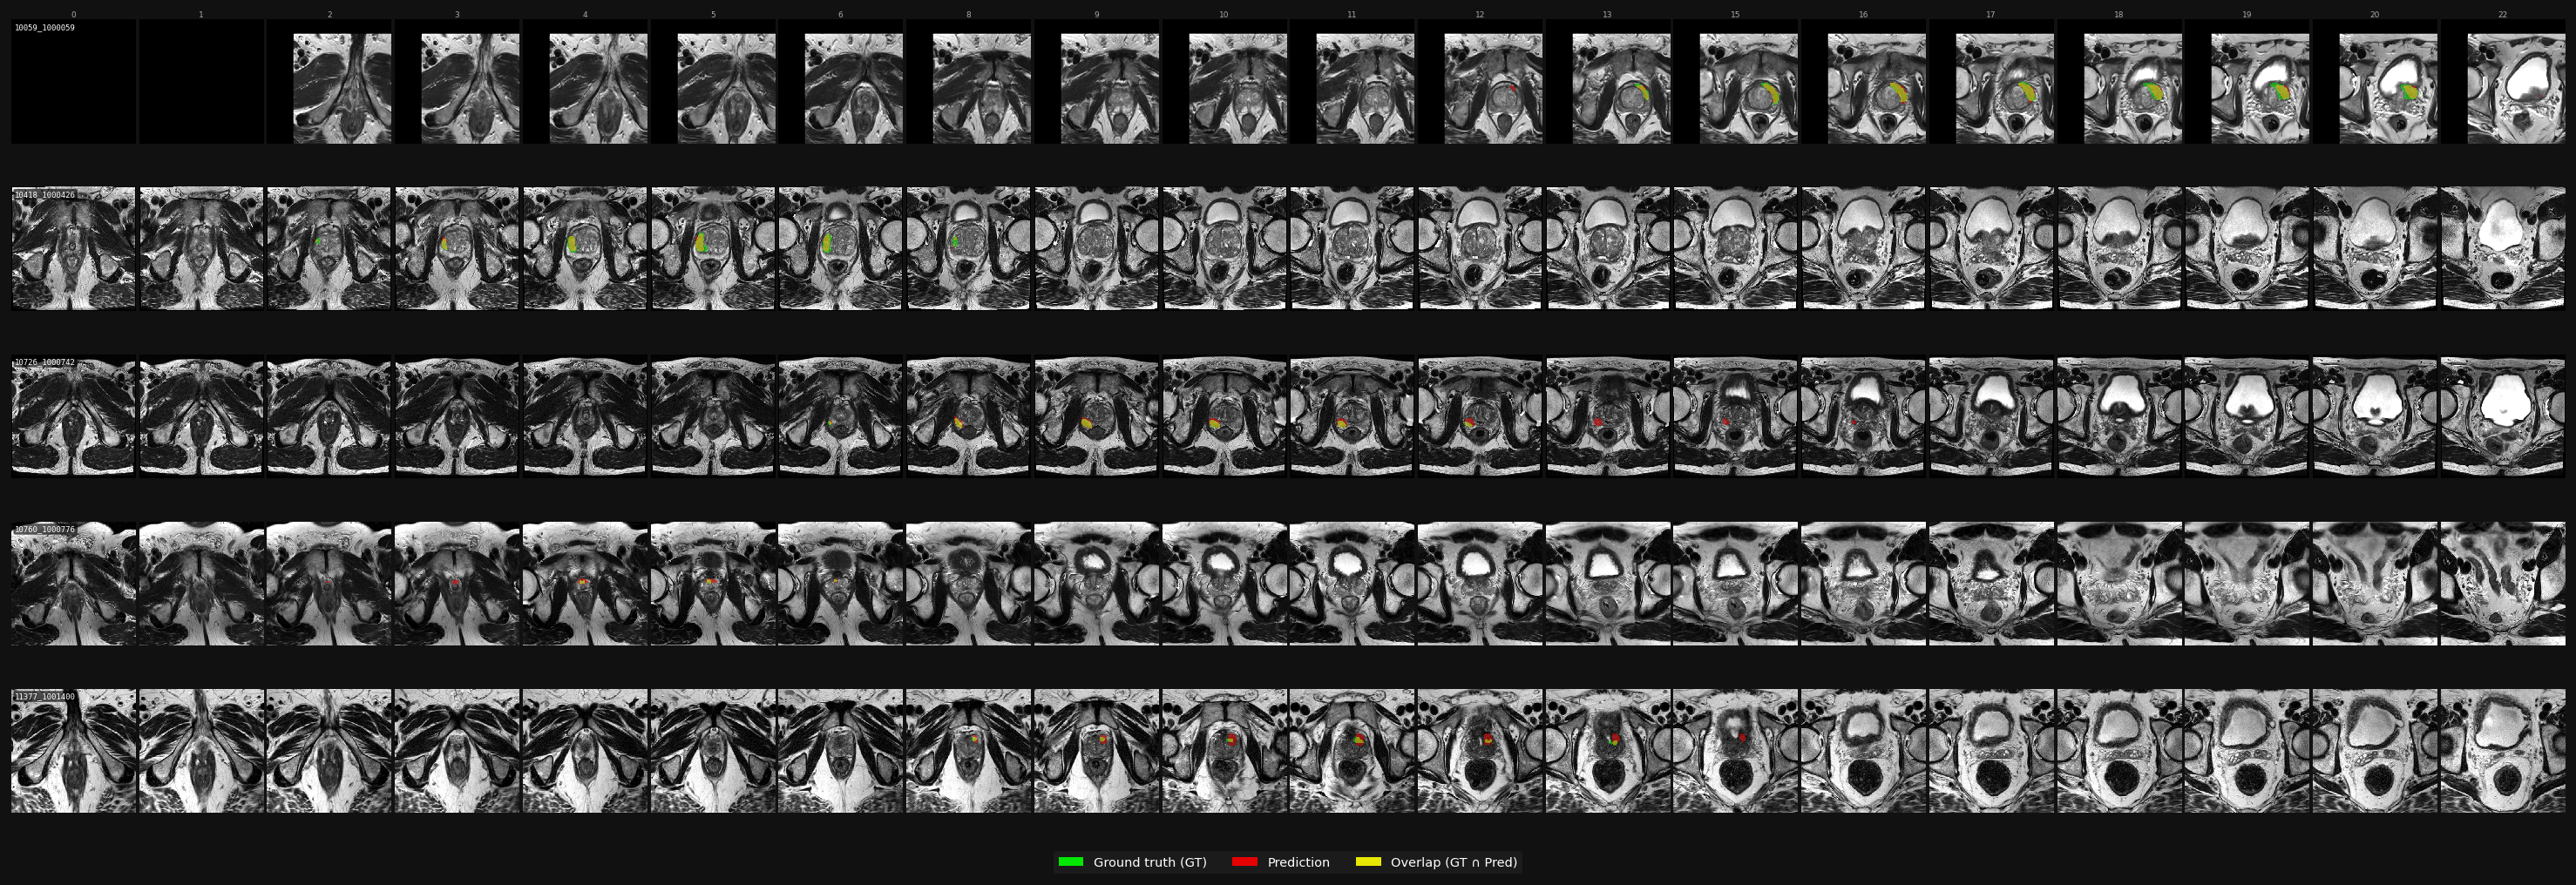
\includegraphics[width=0.78\textwidth]{../visualizations/20260427_221309_unet3d_eval_visualization.png}
\caption{Kvalitativni prikaz evaluacije za Attention U-Net 3D sa SSL inicijalizacijom. \label{fig:attention_ssl_eval}}
\end{figure}

\begin{figure}[H]
\centering
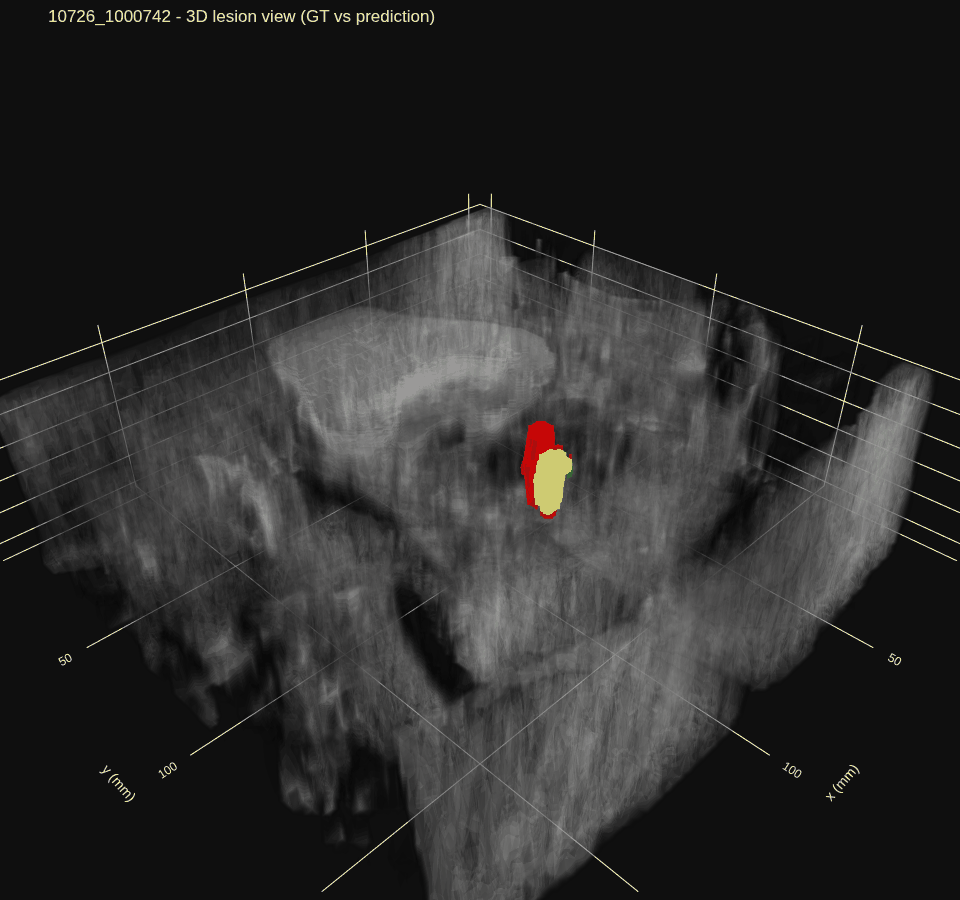
\includegraphics[width=0.78\textwidth]{../visualizations/20260427_221309_unet3d_10726_1000742_t2w_orbit_first_frame.png}
\caption{Primjer 3D prikaza za Attention U-Net 3D sa SSL inicijalizacijom. \label{fig:attention_ssl_3d}}
\end{figure}

\subsection{Deconver}

Deconver je uključen kao alternativna segmentacijska arhitektura s drukčijim mehanizmom miješanja značajki od Attention U-Net polazne arhitekture \cite{deconver}. Rezultati Deconver pokretanja prikazani su u tablici~\ref{tab:deconver_runs}.

\begin{table}[H]
\centering
\scriptsize
\caption{Rezultati Deconver pokretanja. P označava PI-CAI testni skup od 10 slučajeva, a Pr Prostate158 testni skup od 19 slučajeva. \label{tab:deconver_runs}}
\begin{tabular}{>{\raggedright\arraybackslash}p{0.15\textwidth} >{\raggedright\arraybackslash}p{0.20\textwidth} c c c c c c}
\toprule
Pokretanje & Glavna promjena & P-Dice & P-Osj. & P-HD95 & Pr-Dice & Pr-Osj. & Pr-HD95 \\
\midrule
Osnovni Deconver & prva Deconver konfiguracija & \textbf{0.6470} & 0.7732 & \textbf{3.8062} & 0.4591 & 0.5418 & 18.2104 \\
Deconver bez HBV-a & samo T2w i ADC, validacija svakih 5 epoha & 0.6143 & 0.8629 & 12.8735 & 0.4345 & 0.5652 & 21.9676 \\
Deconver A & prilagođen raspored i manja stopa učenja & 0.6452 & 0.7320 & 4.1868 & 0.4703 & 0.4860 & 19.2852 \\
Deconver A + Prostate158 & fino podešavanje na Prostate158 & 0.5030 & \textbf{0.9005} & 99.6676 & 0.4827 & \textbf{0.7158} & 23.1738 \\
Višezadatni Deconver & višezadatna varijanta & 0.6076 & 0.6686 & 4.7500 & \textbf{0.4899} & 0.4942 & \textbf{16.0527} \\
Deconver A + Prostate158 kratko & kraće fino podešavanje na Prostate158 & 0.5118 & 0.9002 & 115.9511 & 0.4895 & 0.6913 & 20.6807 \\
\bottomrule
\end{tabular}
\normalsize
\end{table}

Osnovno Deconver pokretanje daje najbolji PI-CAI Dice i najniži HD95 u ovoj skupini. Konfiguracija Deconver A zadržava vrlo sličan Dice, ali ne poboljšava granice u odnosu na osnovni model. Fino podešavanje na Prostate158 povećava osjetljivost, no na PI-CAI testu dovodi do znatno lošijeg HD95, što upućuje na nestabilnije prostorne predikcije. Slike~\ref{fig:deconver_eval} i~\ref{fig:deconver_3d} prikazuju reprezentativni kvalitativni rezultat osnovnog Deconver modela.

\begin{figure}[H]
\centering
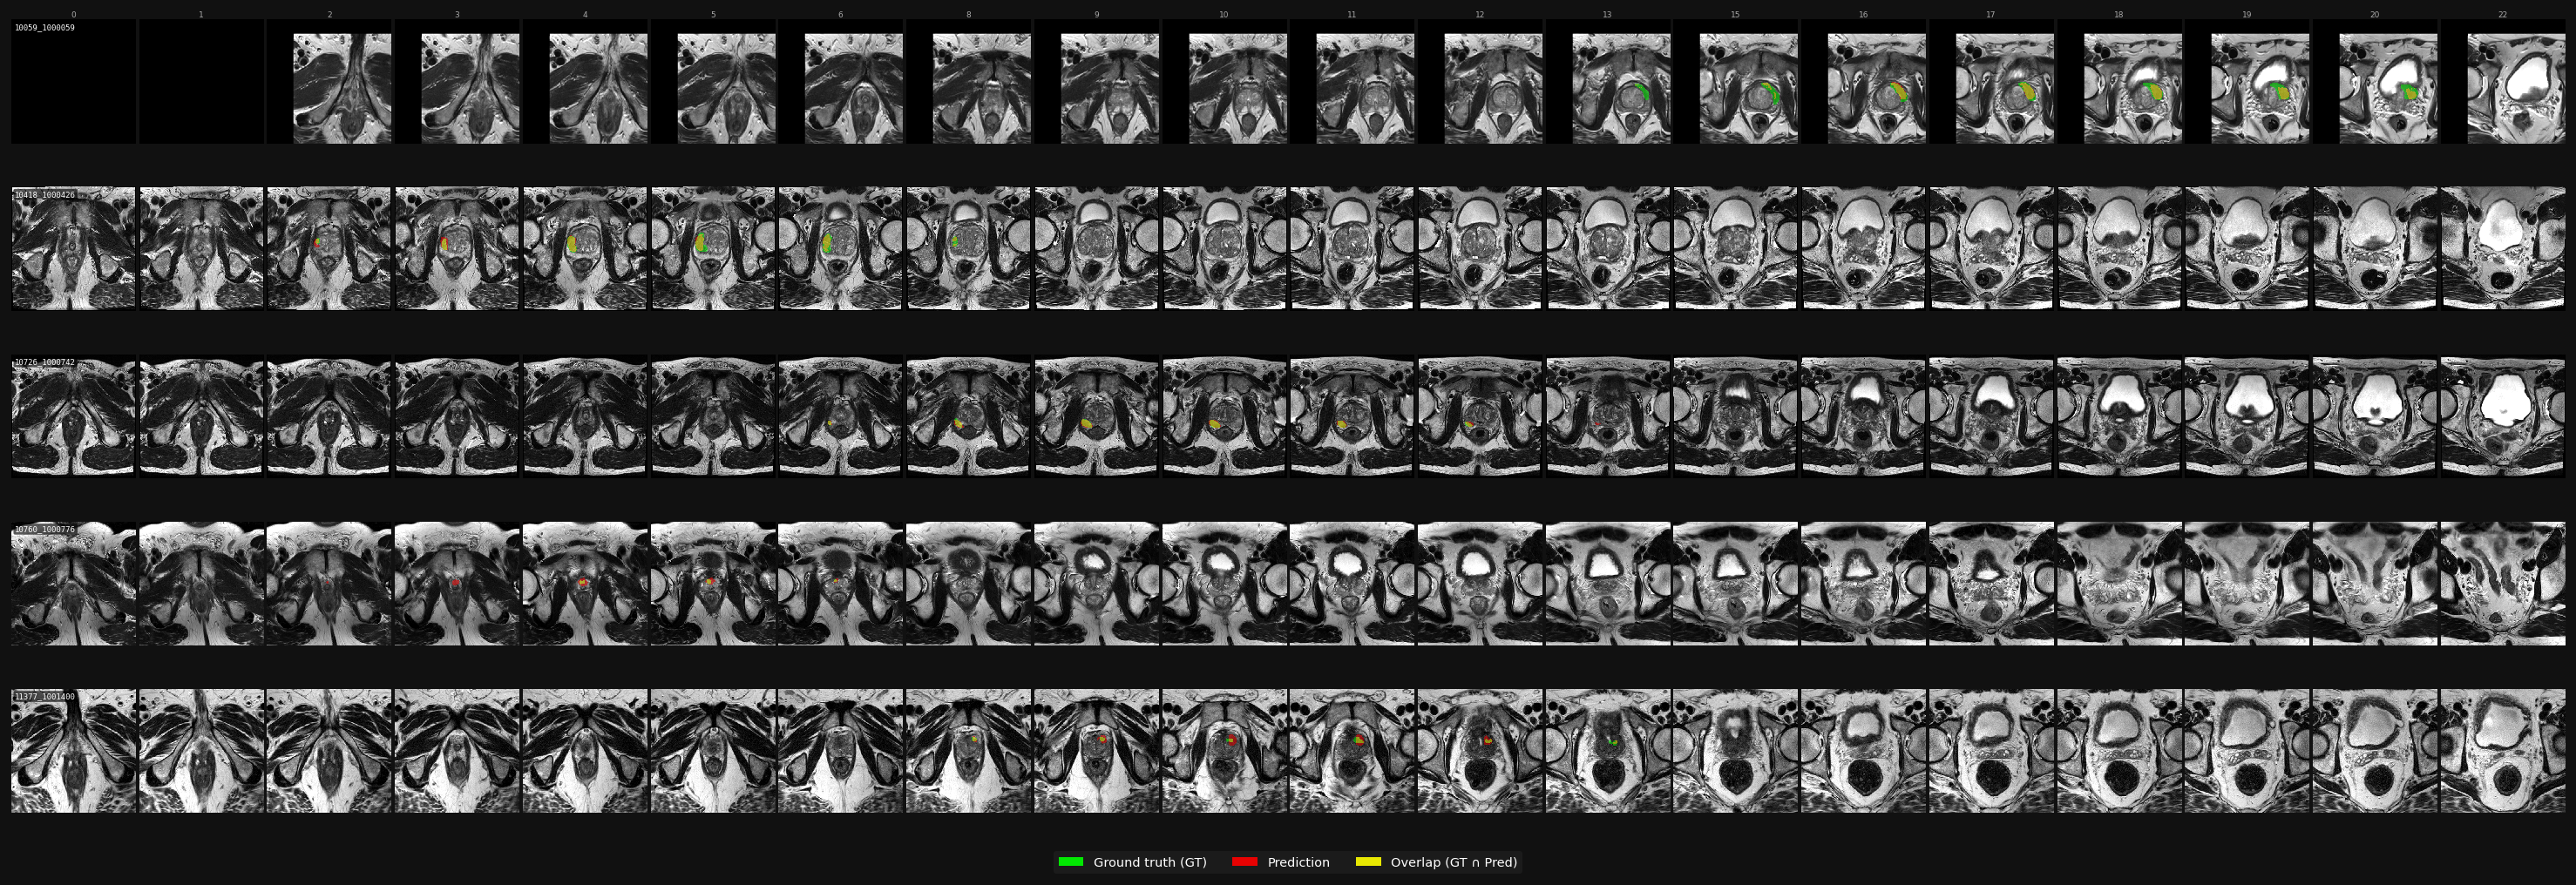
\includegraphics[width=0.78\textwidth]{../visualizations/20260418_224246_deconver_eval_visualization.png}
\caption{Kvalitativni prikaz evaluacije za osnovni Deconver model. \label{fig:deconver_eval}}
\end{figure}

\begin{figure}[H]
\centering
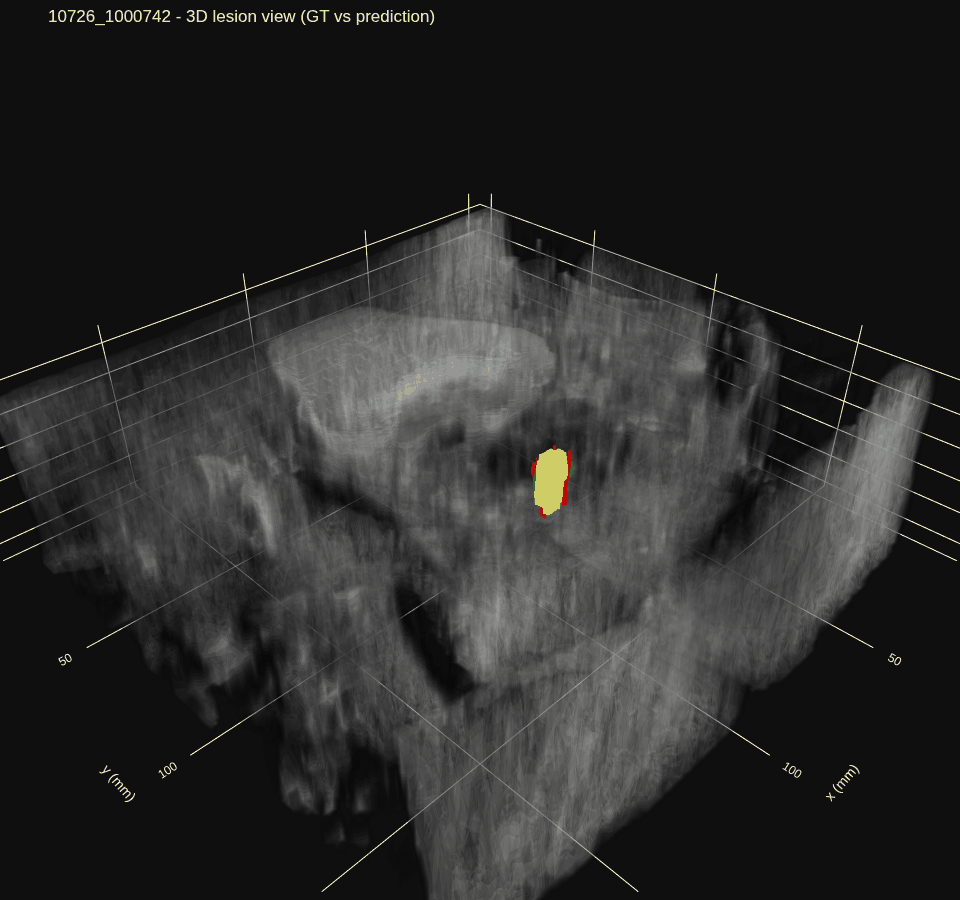
\includegraphics[width=0.78\textwidth]{../visualizations/20260418_224246_deconver_10726_1000742_t2w_orbit_first_frame.png}
\caption{Primjer 3D prikaza za osnovni Deconver model. \label{fig:deconver_3d}}
\end{figure}

\subsection{FCT}

FCT je uključen kao transformatorski nadahnuta usporedba \cite{fct}. Budući da izvorna arhitektura nije razvijena za izravnu 3D obradu volumena, koristi se obrada po aksijalnim presjecima. Sažetak rezultata prikazan je u tablici~\ref{tab:fct_runs}.

\begin{table}[H]
\centering
\scriptsize
\caption{Sažetak FCT pokretanja. P označava PI-CAI testni skup od 10 slučajeva, a Pr Prostate158 testni skup od 19 slučajeva. \label{tab:fct_runs}}
\begin{tabular}{>{\raggedright\arraybackslash}p{0.18\textwidth} >{\raggedright\arraybackslash}p{0.20\textwidth} c c c c c c}
\toprule
Pokretanje & Glavna promjena & P-Dice & P-Osj. & P-HD95 & Pr-Dice & Pr-Osj. & Pr-HD95 \\
\midrule
Osnovni FCT & transformatorski nadahnuta usporedba & \textbf{0.5780} & \textbf{0.5308} & \textbf{4.4900} & \textbf{0.4079} & \textbf{0.4143} & \textbf{34.3002} \\
\bottomrule
\end{tabular}
\normalsize
\end{table}

FCT postiže konkurentan HD95 na PI-CAI testu, ali zaostaje za najboljim Attention i Deconver konfiguracijama prema Diceu i osjetljivosti. Kvalitativni prikaz na slici~\ref{fig:fct_eval} pokazuje tip izlaza koji se dobiva nakon slaganja 2D predikcija u 3D volumen.

\begin{figure}[H]
\centering
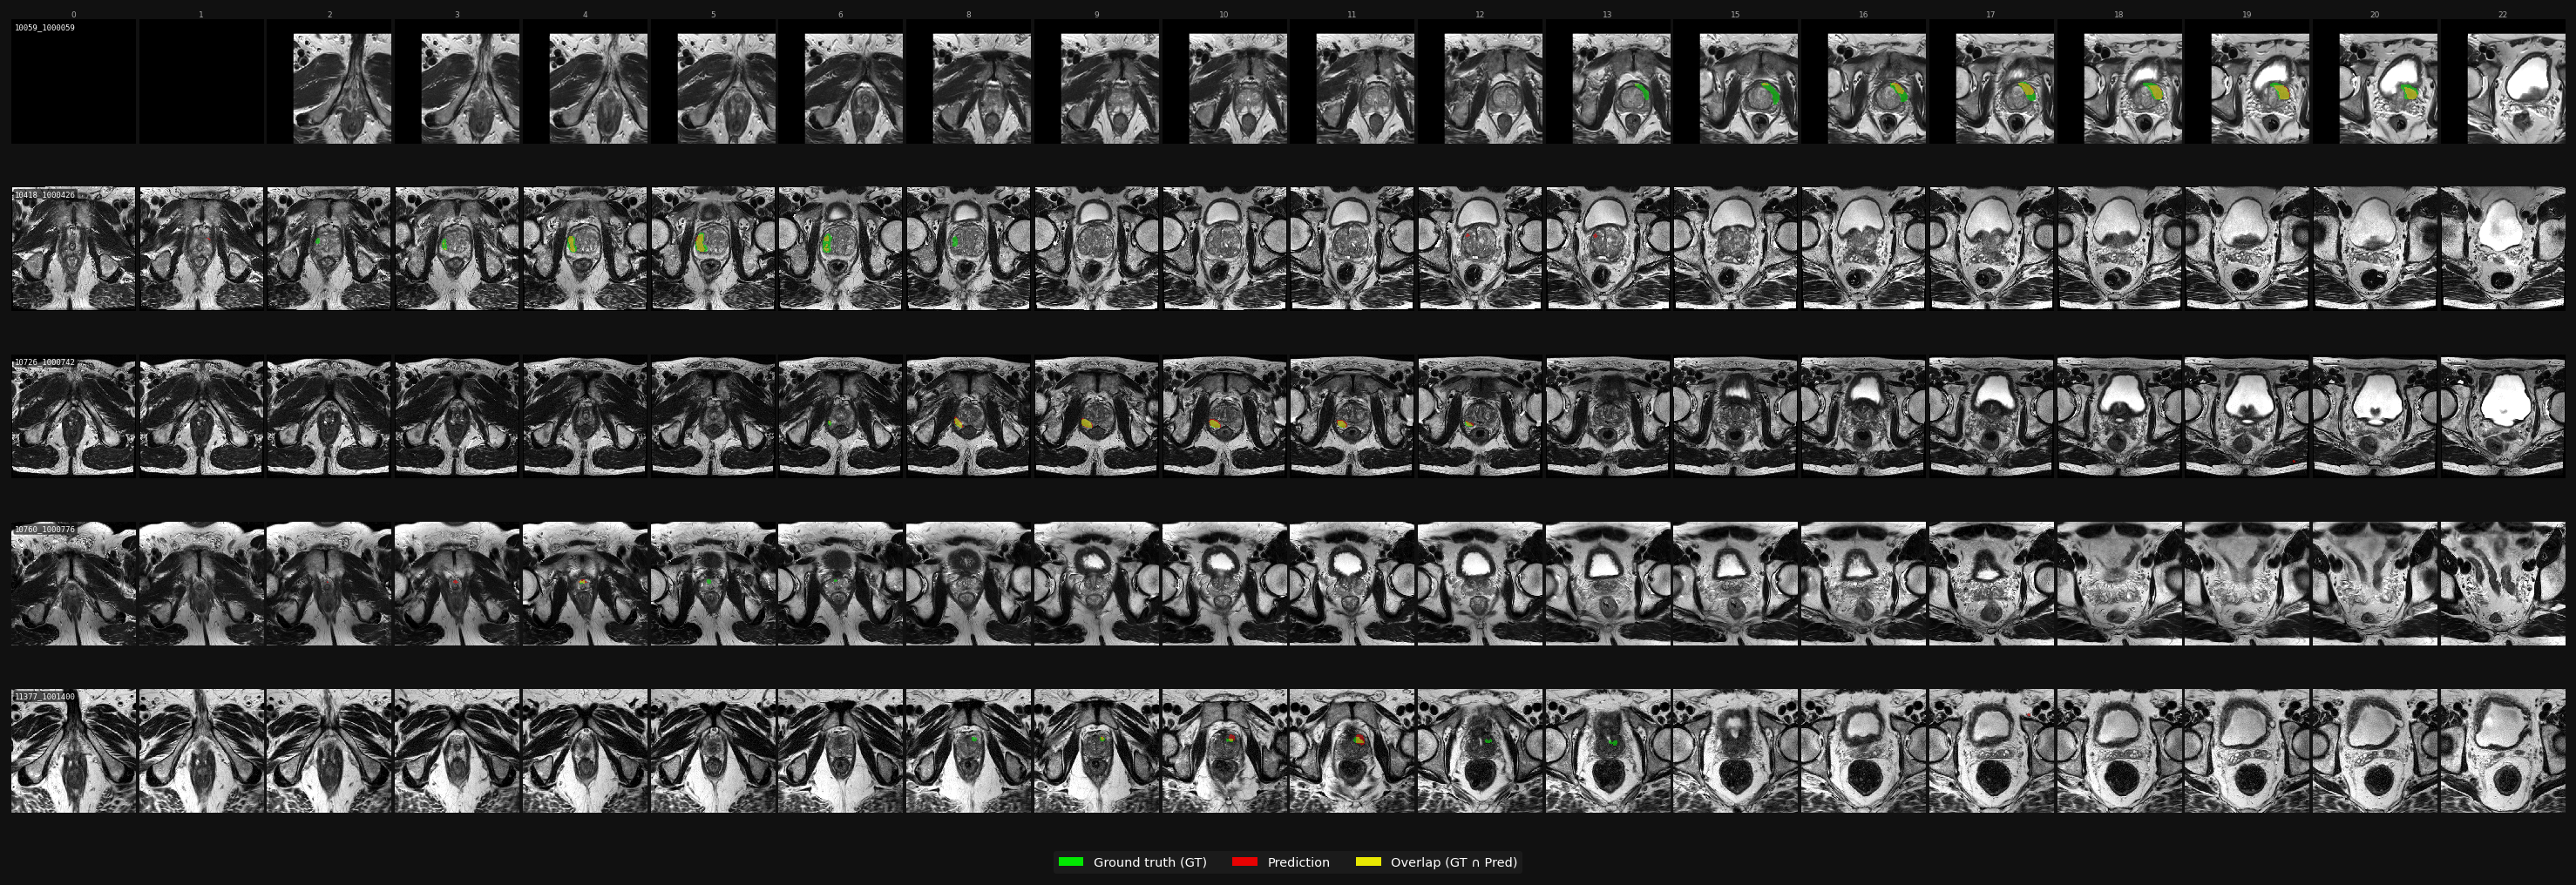
\includegraphics[width=0.78\textwidth]{../visualizations/20260507_205845_fct_default_eval_visualization.png}
\caption{Kvalitativni prikaz evaluacije za FCT model. \label{fig:fct_eval}}
\end{figure}

\subsection{Usporedba reprezentativnih modela}

Tablica~\ref{tab:cross_model} prikazuje sažetu usporedbu reprezentativnih pokretanja na istom fiksnom PI-CAI testnom skupu. Usporedba je ograničena veličinom testnog skupa, ali je korisna za pregled ponašanja arhitektura pod istim evaluacijskim uvjetima.

\begin{table}[H]
\centering
\caption{Usporedba reprezentativnih pokretanja na fiksnom PI-CAI testnom skupu od 10 slučajeva. \label{tab:cross_model}}
\begin{tabular}{>{\raggedright\arraybackslash}p{0.30\textwidth} c c c c}
\toprule
Pokretanje & Komp. & Dice & Osj. & HD95 \\
\midrule
Attention SSL & 0.4409 & 0.6332 & \textbf{0.8329} & 4.4875 \\
Osnovni Deconver & 0.4709 & \textbf{0.6470} & 0.7732 & \textbf{3.8062} \\
Deconver A & \textbf{0.4772} & 0.6452 & 0.7320 & 4.1868 \\
Osnovni FCT & 0.4311 & 0.5780 & 0.5308 & 4.4900 \\
\bottomrule
\end{tabular}
\end{table}

Prema ovom ograničenom skupu rezultata, Deconver je najjača promatrana obitelj modela. Osnovni Deconver model postiže najveći Dice i najniži HD95, dok Deconver A ima najbolji validacijski kompozitni rezultat među reprezentativnim pokretanjima. Attention SSL ostaje konkurentan i postiže najveću osjetljivost, što znači da propušta manje označenih lezija, ali uz nešto slabiju preciznost i graničnu kvalitetu. FCT je koristan kao usporedba s transformatorski nadahnutim pristupom, no u ovom postavu ne nadmašuje najbolje Deconver i Attention konfiguracije.

\subsection{Detekcijske metrike prema PI-CAI postupku}

Segmentacijske metrike u prethodnim tablicama mjere prostorno preklapanje predviđene i stvarne maske, ali ne prikazuju izravno koliko dobro model rangira lezijske kandidate ili cijele slučajeve prema sumnjivosti. Zbog toga je za završnu verziju rada predviđena i dopunska tablica s PI-CAI metrikama rangiranja. U toj tablici AP opisuje rangiranje pojedinačnih lezija, AUROC opisuje rangiranje slučajeva, a kombinirani rezultat računa se kao njihova srednja vrijednost. Te vrijednosti treba prikazati odvojeno od Dicea i HD95 jer odgovaraju drugom pogledu na isti izlaz modela.

\begin{table}[H]
\centering
\caption{Predložak za dopunsku usporedbu modela PI-CAI metrikama rangiranja. \label{tab:picai_ranking_placeholder}}
\begin{tabular}{>{\raggedright\arraybackslash}p{0.34\textwidth} c c c c}
\toprule
Pokretanje & AP & AUROC & PI-CAI rezultat & Broj kandidata \\
\midrule
Attention SSL & TODO & TODO & TODO & TODO \\
Osnovni Deconver & TODO & TODO & TODO & TODO \\
Deconver A & TODO & TODO & TODO & TODO \\
Osnovni FCT & TODO & TODO & TODO & TODO \\
\bottomrule
\end{tabular}
\end{table}

% TODO: Zamijeniti vrijednosti TODO u tablici~\ref{tab:picai_ranking_placeholder} konačnim vrijednostima iz evaluacijskih JSON izvještaja.

\subsection{Analiza po pojedinačnim slučajevima}

Budući da je fiksni PI-CAI testni skup malen, prosječne vrijednosti treba nadopuniti prikazom pojedinačnih slučajeva. Takva tablica treba pokazati razlikuje li se dobar prosjek od dosljednog ponašanja po slučajevima ili od nekoliko vrlo uspješnih predikcija. Posebno je važno uključiti negativne slučajeve jer oni ne ulaze u prosjeke Dicea, IoU-a, osjetljivosti i preciznosti, ali su ključni za procjenu lažno pozitivnog ponašanja modela.

\begin{table}[H]
\centering
\scriptsize
\caption{Predložak za analizu ponašanja modela po slučajevima na fiksnom PI-CAI testnom skupu. \label{tab:per_case_placeholder}}
\setlength{\tabcolsep}{2pt}
\begin{tabular}{>{\raggedright\arraybackslash}p{0.15\textwidth}
                >{\raggedright\arraybackslash}p{0.15\textwidth}
                >{\centering\arraybackslash}p{0.10\textwidth}
                >{\centering\arraybackslash}p{0.12\textwidth}
                >{\centering\arraybackslash}p{0.08\textwidth}
                >{\raggedright\arraybackslash}p{0.22\textwidth}}
\toprule
Pokretanje & Slučaj & Ref. lezija & Pred. poz. voksela & Dice & Napomena \\
\midrule
TODO & TODO & da/ne & TODO & TODO & TODO: npr. pogodak, promašaj, lažno pozitivno \\
\bottomrule
\end{tabular}
\normalsize
\end{table}

% TODO: Popuniti tablicu~\ref{tab:per_case_placeholder} za reprezentativne modele ili za najbolji odabrani model: oznaka pozitivnog/negativnog slučaja, broj predviđenih pozitivnih voksela, Dice za pozitivne slučajeve i napomena o lažno pozitivnim predikcijama na negativnim slučajevima.

\subsection{Ograničenja rezultata i ponašanje na negativnim slučajevima}

Rezultati u tablicama trebaju se tumačiti zajedno s načinom agregacije metrika. Dice, IoU, osjetljivost i preciznost računaju se samo nad slučajevima koji imaju pozitivnu referentnu masku, dok negativni slučajevi ne ulaze u te prosjeke. Takav postupak sprječava da potpuno prazni negativni slučajevi umjetno povećaju prosječni Dice, ali znači da tablice same po sebi ne prikazuju sklonost modela lažno pozitivnim predikcijama na negativnim slučajevima. Budući da fiksni PI-CAI testni skup sadrži 5 negativnih slučajeva, ta je provjera važna za tumačenje modela.

Kvalitativni prikazi evaluacije zato imaju ulogu dopune numeričkim metrikama. Ako model na negativnom slučaju predvidi leziju, to se neće odraziti kroz Dice prosjek pozitivnih slučajeva, ali je bitno za ukupno ponašanje sustava. U ovom izdanju rada još nije dodana zasebna tablica s brojem lažno pozitivnih negativnih slučajeva po modelu.

% TODO: Nakon popunjavanja tablice po slučajevima, u ovom odlomku sažeti broj negativnih slučajeva s lažno pozitivnom predikcijom za svaki reprezentativni model.

Usporedba PI-CAI i Prostate158 rezultata pokazuje pad ili promjenu ponašanja na vanjskom skupu. To je očekivano s obzirom na razliku u izvoru podataka, organizaciji modaliteta i činjenicu da se DWI u Prostate158 koristi kao zamjena za HBV kanal. Ipak, broj Prostate158 testnih slučajeva je malen, pa se iz tih rezultata ne može izvesti općenit zaključak o generalizaciji modela. Oni služe kao upozorenje da dobro ponašanje na jednom skupu ne znači automatski jednako ponašanje na drugom.

Evaluacijski postupak pretvara logite u binarnu masku sigmoidnom funkcijom i pragom 0,5. U kodu postoji opcionalno uklanjanje malih povezanih komponenti iz predikcije, ali prikazani rezultati nisu organizirani kao zasebna usporedba s i bez takvog postprocesiranja. Zbog toga se u raspravi ne tvrdi da postprocesiranje poboljšava rezultate. Ako se u završnoj verziji rada bude koristio postprocesirani izlaz, potrebno je navesti prag, minimalni volumen komponente, povezanost komponenti i usporedbu s osnovnom evaluacijom.

% TODO: Ako se uključe rezultati podešavanja postprocesiranja, dodati tablicu s pragom, minimalnim volumenom komponente, povezanosti i učinkom na PI-CAI i Prostate158 metrike.

Krivulje treniranja i validacije nisu uključene u ovo poglavlje jer u trenutnoj verziji rada nisu izdvojene kao slike. One bi bile korisne za prikaz stabilnosti učenja, osobito kod ranih Attention U-Net pokretanja s visokom osjetljivošću i niskom preciznošću.

% TODO: Dodati TensorBoard krivulje ili izvezene grafove validacijskog Dicea, osjetljivosti i kompozitnog rezultata za reprezentativna pokretanja.

\section{OBJAŠNJIVOST MODELA}

Objašnjiva umjetna inteligencija, odnosno XAI, u ovom je radu korištena kao dopunska analiza uz numeričke metrike evaluacije. Dice, IoU, HD95, preciznost i osjetljivost sažimaju podudaranje predviđene i stvarne maske, ali ne pokazuju izravno na koje se dijelove volumena model oslanja pri izračunu predikcije. Zbog toga su za odabrani primjer izrađene tri vrste objašnjenja: Grad-CAM, mape osjetljivosti i ablacija modaliteta. Takvi postupci pripadaju širem području \textit{post-hoc} objašnjenja modela, u kojem se već istrenirani model analizira bez promjene njegove arhitekture ili ponovnog treniranja \cite{xai_survey}.

Važno je razlikovati evaluaciju segmentacijske kvalitete od objašnjenja ponašanja modela. Numerička metrika odgovara na pitanje koliko se predikcija podudara s referentnom oznakom, dok XAI vizualizacija pokušava prikazati koji su dijelovi ulaza ili koji su modaliteti bili utjecajni za konkretni izlaz. Dobra vrijednost metrike ne znači nužno da se model oslanja na klinički smislen signal, a uvjerljiva toplinska karta (engl. \textit{heat map}) sama po sebi ne dokazuje ispravnost segmentacije. U ovom poglavlju XAI se zato tumači kao kvalitativni alat za provjeru i opis ponašanja modela, a ne kao zaseban dokaz kliničke pouzdanosti.

Grad-CAM polazi od odabranog skalarnog izlaza modela i propagira gradijente prema izabranom sloju značajki \cite{gradcam}. Ako $A^k$ označuje $k$-tu mapu značajki u tom sloju, a $y$ ciljni skalarni izlaz, težina te mape računa se prostornim uprosječivanjem gradijenta:
\[
\alpha_k = \frac{1}{Z}\sum_i\sum_j\sum_l \frac{\partial y}{\partial A^k_{ijl}},
\]
gdje $Z$ označuje broj prostornih položaja u mapi značajki. Završna Grad-CAM karta dobiva se kao pozitivni dio ponderirane sume mapa značajki,
\[
L_{\mathrm{Grad-CAM}} = \operatorname{ReLU}\left(\sum_k \alpha_k A^k\right).
\]
U ovom radu ta je karta izračunata u 3D području interesa i zatim interpolirana na prostornu rezoluciju analiziranog isječka volumena, pa prikazuje grubu lokalizaciju regija koje su u odabranom sloju najviše pridonijele ciljnom izlazu.

Za prikaz na slici~\ref{fig:xai_gradcam} korišten je osnovni Deconver model, slučaj 10726\_1000742, ulazni modaliteti T2w, ADC i HBV te sloj \texttt{encoder.blocks.3}. Ciljni izlaz definiran je iz segmentacijske predikcije modela, a izračun je ograničen na područje interesa oko predviđene ili označene lezije kako bi se smanjilo memorijsko opterećenje i prikaz usmjerio na relevantni dio volumena.

\begin{figure}[H]
\centering
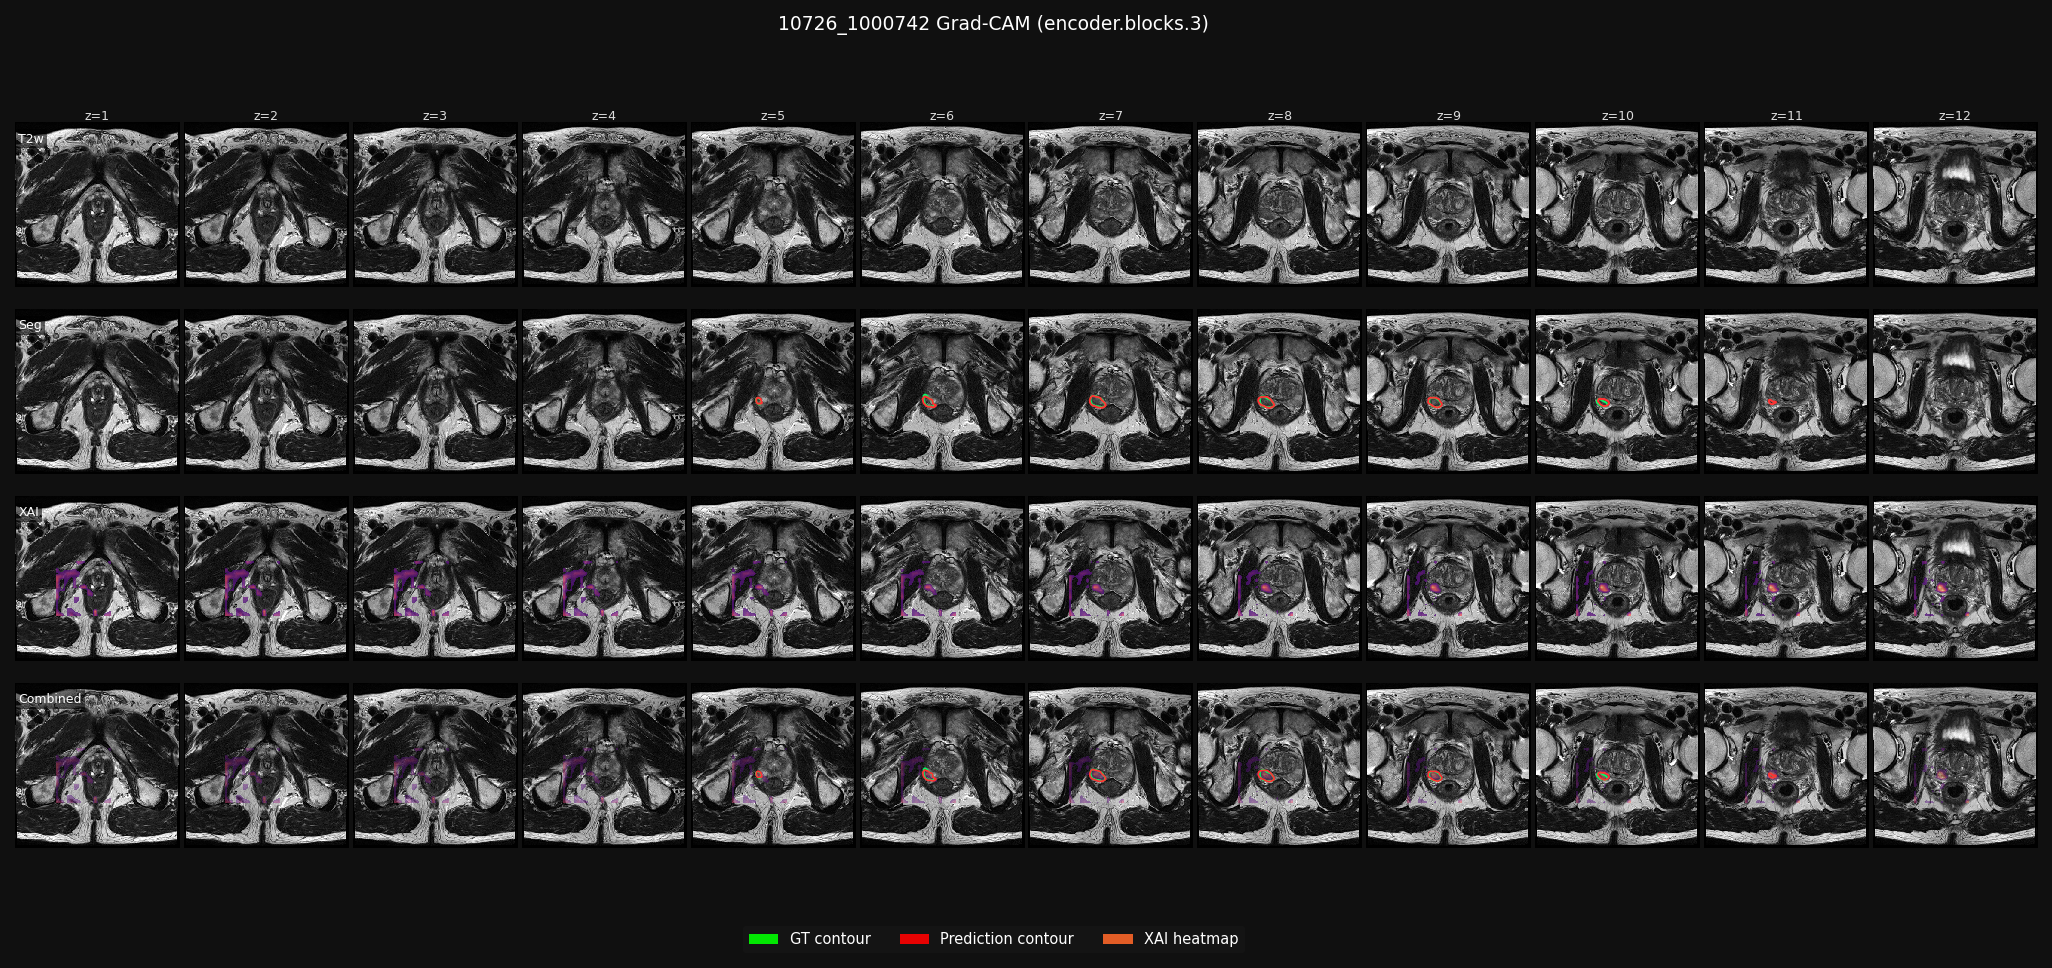
\includegraphics[width=0.78\textwidth]{../visualizations/xai/20260418_224246_deconver_10726_1000742_gradcam.png}
\caption{Primjer Grad-CAM objašnjenja za osnovni Deconver model. \label{fig:xai_gradcam}}
\end{figure}

Slika~\ref{fig:xai_gradcam} prikazuje T2w presjeke, konture referentne i predviđene maske te toplinsku kartu Grad-CAM objašnjenja. Takav prikaz pomaže provjeriti nalazi li se aktivacija u blizini predviđene lezije ili izvan nje. Budući da Grad-CAM karta ovisi o odabranom sloju i ima grublju rezoluciju od ulaznog volumena, iz nje se ne smije zaključivati precizna granica lezije niti klinička ispravnost predikcije.

Mape osjetljivosti temelje se na gradijentu ciljnog izlaza u odnosu na ulazne voksele \cite{simonyan_saliency}. Za ulazni volumen $x$ i ciljni izlaz $y$ osnovna se mapa može zapisati kao
\[
S(x)=\left|\frac{\partial y}{\partial x}\right|.
\]
Veća apsolutna vrijednost gradijenta znači da bi mala promjena pripadnog ulaznog voksela, prema lokalnoj linearnoj aproksimaciji modela, jače promijenila ciljni izlaz. Budući da je ulaz multimodalan, osjetljivost se može promatrati objedinjeno preko svih kanala ili odvojeno za T2w, ADC i HBV. Objedinjena karta u ovom radu dobivena je iz najveće normalizirane osjetljivosti po modalitetima na istom prostornom položaju.

Slika~\ref{fig:xai_saliency} prikazuje objedinjenu mapu osjetljivosti i pojedinačne mape po modalitetima za isti Deconver izlaz. Redak s objedinjenom mapom pokazuje prostorne položaje na kojima je izlaz lokalno najosjetljiviji na promjene ulaza, dok modalitetni redci pomažu uočiti razlikuje li se osjetljivost između T2w, ADC i HBV kanala.

\begin{figure}[H]
\centering
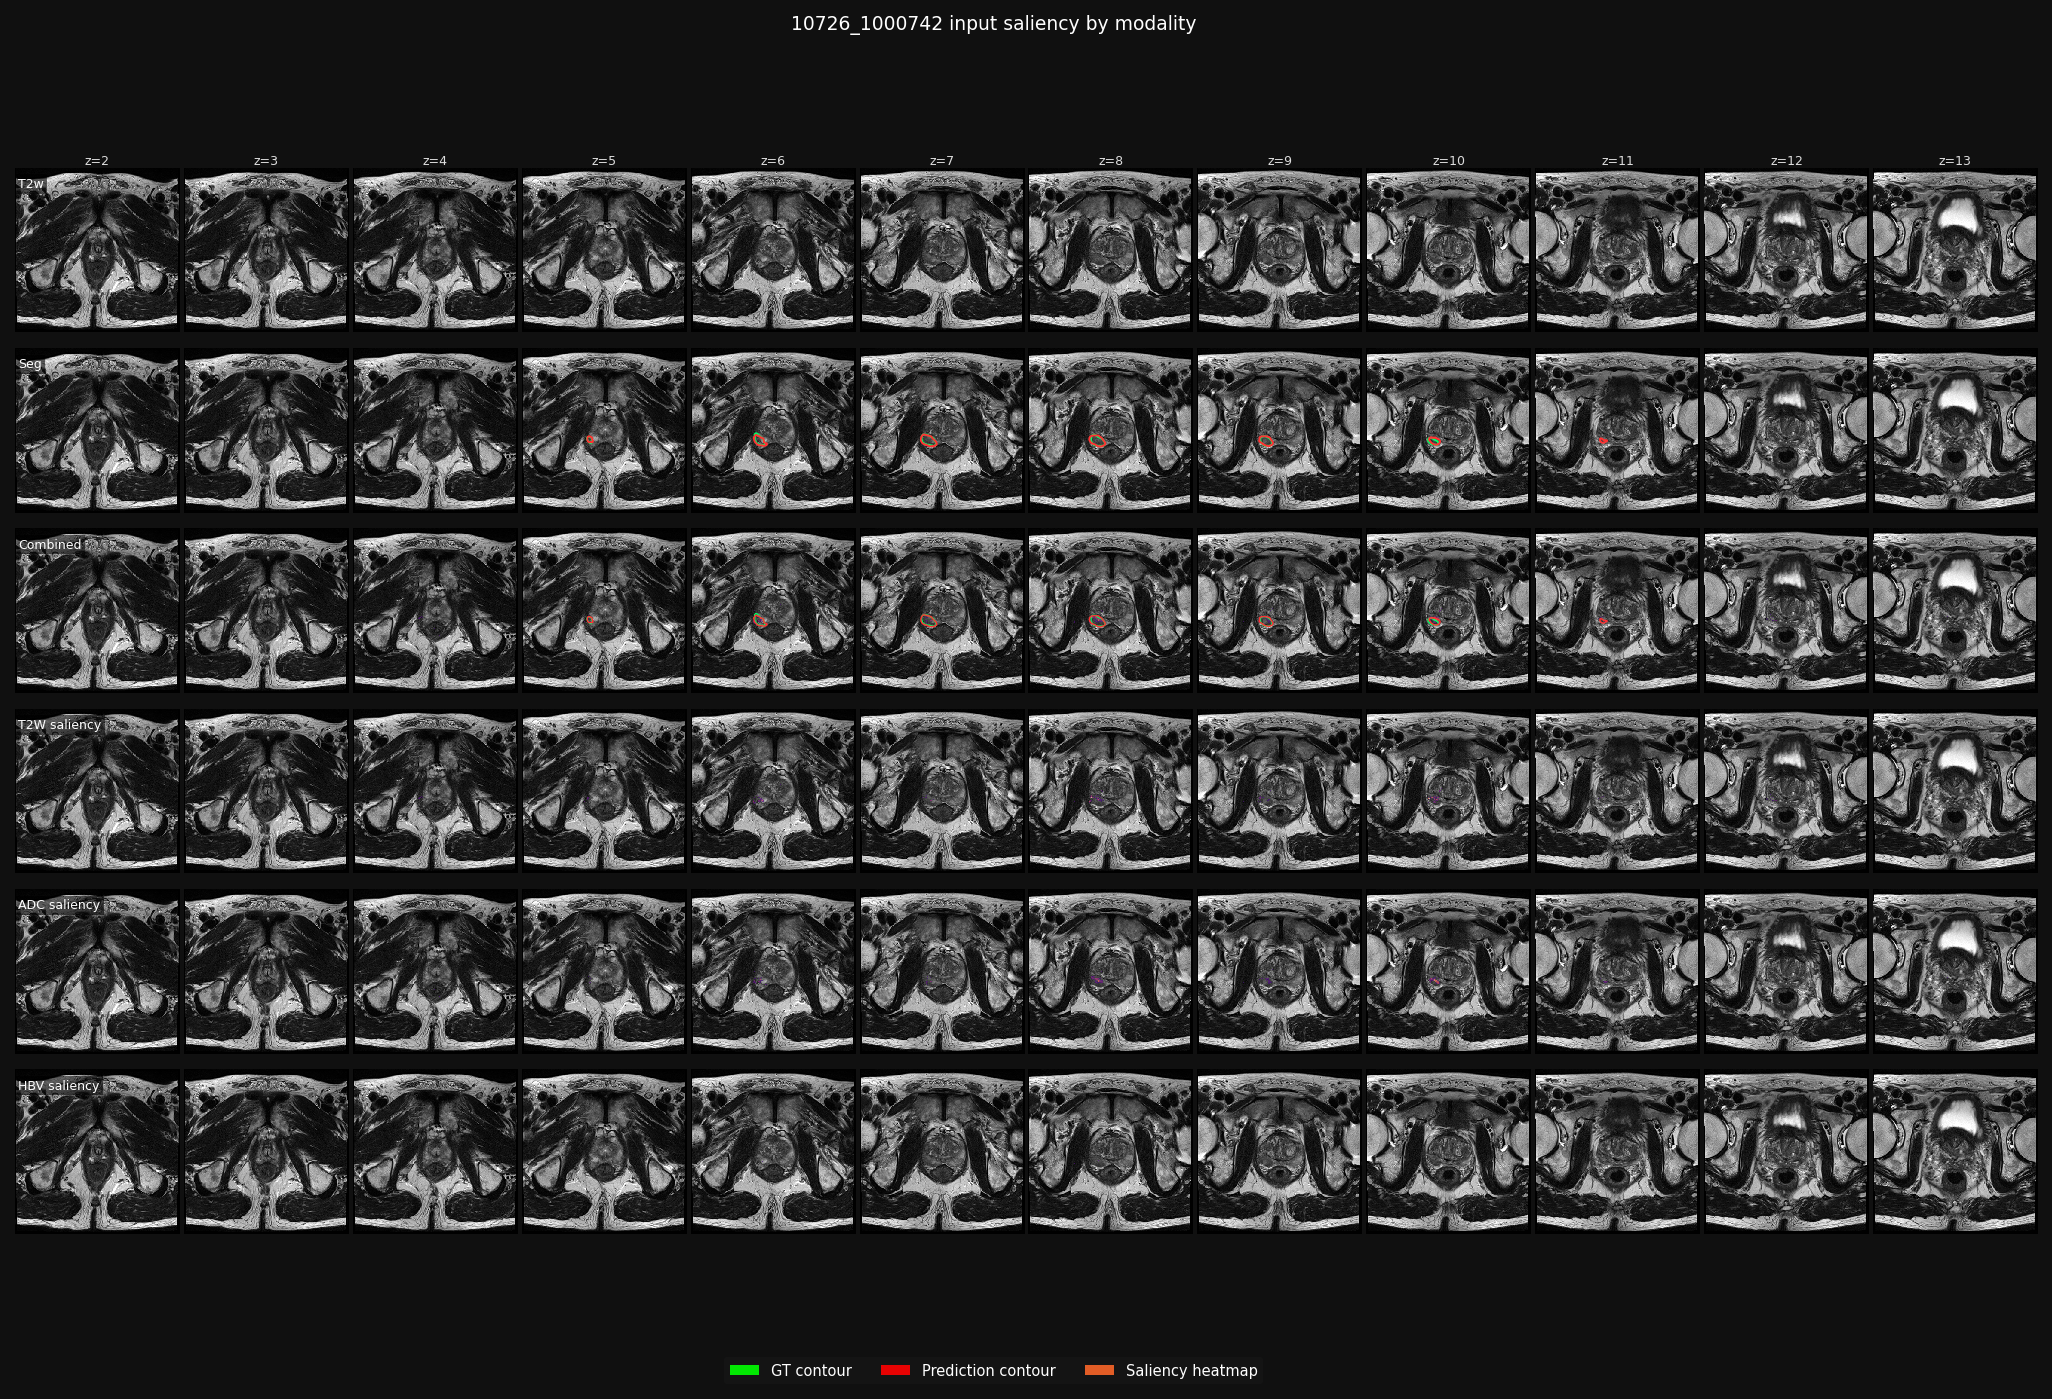
\includegraphics[width=0.78\textwidth]{../visualizations/xai/20260418_224246_deconver_10726_1000742_saliency.png}
\caption{Primjer objedinjene mape osjetljivosti za osnovni Deconver model. \label{fig:xai_saliency}}
\end{figure}

Mape osjetljivosti treba čitati oprezno jer prikazuju lokalnu derivaciju, a ne nužno stvarni uzročno-posljedični doprinos pojedinog anatomskog područja. One mogu biti šumovite i osjetljive na normalizaciju, odabrani ciljni izlaz i arhitekturu modela. Zbog toga su korisne za usporedbu obrazaca osjetljivosti, ali nisu dovoljne za tvrdnju da je model prepoznao leziju na način koji bi odgovarao radiološkom obrazloženju.

Ablacija modaliteta nadopunjuje gradijentne metode jednostavnom intervencijskom provjerom. U toj analizi jedan se ulazni kanal postavlja na nulu, dok ostali modaliteti ostaju nepromijenjeni. Zatim se ponovno računa segmentacija i uspoređuju se metrika predikcije, broj predviđenih voksela i prosječni pad vjerojatnosti u području osnovne predikcije. Ako uklanjanje nekog modaliteta snažno smanji vjerojatnosti ili ukloni predviđenu masku, to upućuje na veću ovisnost konkretne predikcije o tom modalitetu. Takav zaključak vrijedi za analizirani slučaj i zadani model, a ne kao opća tvrdnja o važnosti modaliteta u svim podacima.

Sažetak ablacije modaliteta za isti slučaj prikazan je na slici~\ref{fig:xai_ablation}. U prikazanom primjeru uklanjanje ADC i HBV kanala dovodi do snažnog pada vjerojatnosti u području osnovne predikcije i nestanka predviđene maske, dok uklanjanje T2w kanala ne uklanja predikciju, nego mijenja njezin opseg i metrike. To upućuje na to da se konkretni Deconver izlaz u ovom slučaju više oslanjao na difuzijske modalitete nego na T2w kanal, ali taj zaključak ostaje ograničen na opisano pokretanje, slučaj i način ablacijske provjere.

\begin{figure}[H]
\centering
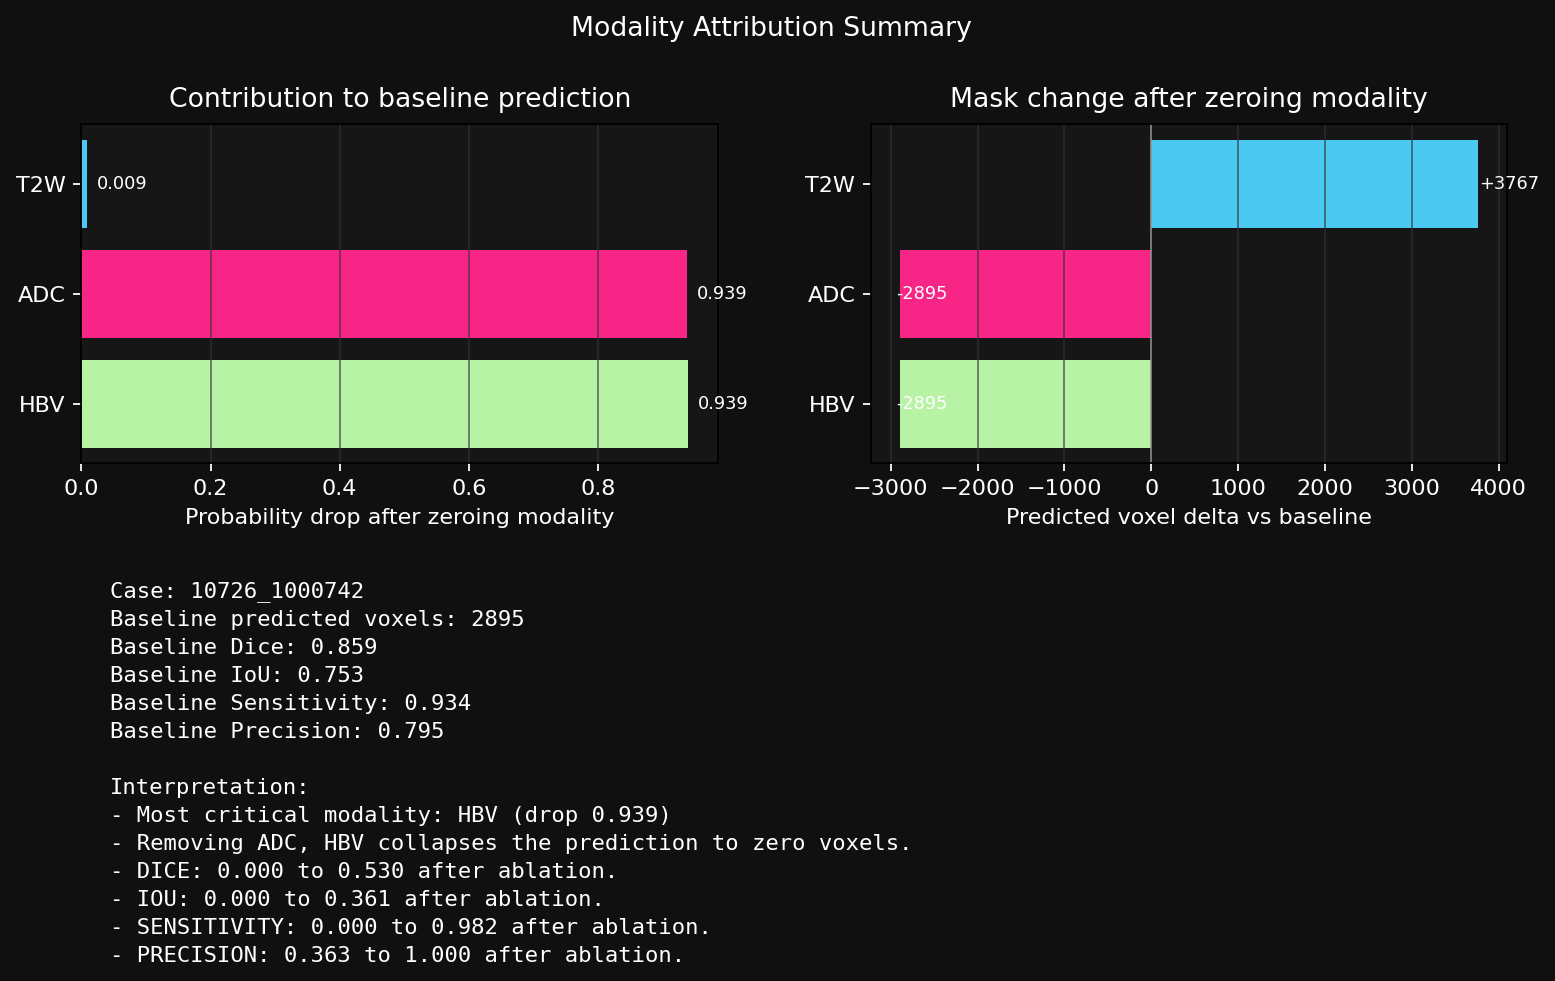
\includegraphics[width=0.78\textwidth]{../visualizations/xai/20260418_224246_deconver_10726_1000742_modality_ablation_summary.png}
\caption{Primjer sažetka ablacije modaliteta za osnovni Deconver model. \label{fig:xai_ablation}}
\end{figure}

Glavno ograničenje prikazanih XAI rezultata proizlazi iz njihove \textit{post-hoc} naravi. Grad-CAM, mape osjetljivosti i ablacija modaliteta ne objašnjavaju model u potpunosti, nego daju djelomične poglede na njegovo ponašanje za jedan ulaz i jednu kontrolnu točku. Posebno kod mapa osjetljivosti poznato je da vizualno uvjerljive karte mogu biti nedovoljno osjetljive na stvarno naučene parametre ili podatke, zbog čega su potrebne provjere razumnosti i oprezna interpretacija \cite{adebayo_sanity}. U ovom radu XAI prikazi služe za kvalitativnu analizu i otkrivanje mogućih obrazaca oslanjanja modela na modalitete, dok se zaključci o segmentacijskoj kvaliteti i dalje temelje na evaluacijskim metrikama, kvalitativnim prikazima segmentacije i jasno navedenim ograničenjima testnih skupova.

\section{ZAKLJUČAK}

U radu je prikazan sustav za automatsku segmentaciju suspektnih lezija prostate iz multimodalnih MR snimki. Sustav obuhvaća učitavanje PI-CAI i Prostate158 podataka, registraciju i normalizaciju modaliteta, nadzirano treniranje volumetrijskih modela, samonadzirano predtreniranje enkodera, evaluaciju spremljenih kontrolnih točaka, kvalitativnu vizualizaciju i osnovne metode objašnjivosti.

Na fiksnom PI-CAI testnom skupu od 10 slučajeva osnovni Deconver model postiže najbolji Dice, s vrijednošću 0.6470, dok Attention U-Net sa SSL inicijalizacijom postiže najveću osjetljivost među reprezentativnim modelima. Na dodatnom Prostate158 testnom skupu rezultati su niži i pokazuju da se ponašanje modela mijenja pri prijelazu na drugi skup podataka. To ograničava zaključke i upućuje na potrebu za širim vanjskim vrednovanjem prije bilo kakvog praktičnog tumačenja.

Glavna ograničenja rada su mali fiksni PI-CAI testni skup, ograničen broj Prostate158 testnih slučajeva, osjetljivost rezultata na odabir validacijskog kriterija i nepotpuno pokrivena teorijska literatura. Budući rad može uključiti strože vanjsko vrednovanje, dodatne višezadatne modele, korištenje segmentacije prostate za prostorno ograničavanje područja interesa i usporedbu s dodatnim arhitekturama, ali takve nadogradnje treba evaluirati odvojeno od rezultata prikazanih u ovom radu.

\newpage
\addcontentsline{toc}{section}{LITERATURA}
\bibliographystyle{unsrt}
\bibliography{./supp_files/bibtex_baza}

\newpage
\section*{Popis oznaka}
\addcontentsline{toc}{section}{Popis oznaka}

\begin{tabular}{>{\raggedright\arraybackslash}p{0.18\textwidth} >{\raggedright\arraybackslash}p{0.72\textwidth}}
$P$ & predviđena binarna segmentacijska maska \\
$T$ & referentna binarna segmentacijska maska \\
$TP$ & broj istinito pozitivnih voksela \\
$FP$ & broj lažno pozitivnih voksela \\
$FN$ & broj lažno negativnih voksela \\
$A^k$ & $k$-ta mapa značajki u odabranom sloju modela \\
$\alpha_k$ & težina $k$-te mape značajki u Grad-CAM postupku \\
$Z$ & broj prostornih položaja u mapi značajki \\
\end{tabular}

\newpage
\section*{Popis kratica}
\addcontentsline{toc}{section}{Popis kratica}

\begin{tabular}{>{\raggedright\arraybackslash}p{0.18\textwidth} >{\raggedright\arraybackslash}p{0.72\textwidth}}
ADC & karta prividnog difuzijskog koeficijenta, engl. \textit{Apparent Diffusion Coefficient} \\
AP & prosječna preciznost, engl. \textit{Average Precision} \\
AUROC & površina ispod ROC krivulje, engl. \textit{Area Under the Receiver Operating Characteristic Curve} \\
BCE & binarna unakrsna entropija, engl. \textit{Binary Cross-Entropy} \\
DWI & difuzijski ponderirana snimka, engl. \textit{Diffusion-Weighted Imaging} \\
FCT & \textit{Fully Convolutional Transformer} \\
Grad-CAM & gradijentno ponderirana aktivacijska karta klase, engl. \textit{Gradient-weighted Class Activation Mapping} \\
HBV & difuzijski ponderirana snimka visoke b-vrijednosti, engl. \textit{High b-value} \\
HD95 & 95. percentil Hausdorffove udaljenosti \\
IoU & omjer presjeka i unije, engl. \textit{Intersection over Union} \\
MR & magnetska rezonancija \\
PI-CAI & \textit{Prostate Imaging: Cancer AI} \\
PI-RADS & \textit{Prostate Imaging Reporting and Data System} \\
ROI & područje interesa, engl. \textit{Region of Interest} \\
SSL & samonadzirano učenje, engl. \textit{Self-Supervised Learning} \\
T2w & T2-mjerena snimka, engl. \textit{T2-weighted} \\
XAI & objašnjiva umjetna inteligencija, engl. \textit{Explainable Artificial Intelligence} \\
\end{tabular}

\newpage
\section*{Sažetak}
\addcontentsline{toc}{section}{Sažetak}

U radu je prikazan sustav za automatsku segmentaciju suspektnih lezija prostate iz multimodalnih MR snimki primjenom dubokog učenja. Sustav koristi T2w, ADC i HBV modalitete, provodi registraciju i normalizaciju volumena te trenira više segmentacijskih arhitektura, uključujući Attention U-Net 3D, Deconver i FCT. Evaluacija je provedena na fiksnom PI-CAI testnom skupu od 10 slučajeva i dodatnom Prostate158 testnom skupu od 19 slučajeva. Osnovni Deconver model postiže najbolji Dice na PI-CAI testu, dok Attention U-Net sa samonadziranom inicijalizacijom postiže najveću osjetljivost među reprezentativnim modelima. Rezultati pokazuju da modeli mogu segmentirati dio suspektnih lezija, ali su zaključci ograničeni veličinom testnih skupova i razlikama između izvora podataka.

\bigskip
\noindent\textbf{Ključne riječi:} Attention U-Net, Deconver, duboko učenje, magnetska rezonancija prostate, segmentacija medicinskih slika

\newpage
\section*{Abstract}
\addcontentsline{toc}{section}{Abstract}

\noindent\textbf{Automatic segmentation of suspicious prostate lesions from multimodal MRI using deep learning}

This thesis presents a system for automatic segmentation of suspicious prostate lesions from multimodal MRI using deep learning. The system uses T2w, ADC, and HBV modalities, performs registration and intensity normalization, and trains several segmentation architectures, including Attention U-Net 3D, Deconver, and FCT. Evaluation was performed on a fixed 10-case PI-CAI test set and an additional 19-case Prostate158 test set. The baseline Deconver model achieved the best Dice score on the PI-CAI test set, while the Attention U-Net model with self-supervised initialization achieved the highest sensitivity among the representative models. The results indicate that the models can segment some suspicious lesions, but the conclusions are limited by the size of the test sets and by differences between data sources.

\bigskip
\noindent\textbf{Keywords:} Attention U-Net, Deconver, deep learning, medical image segmentation, prostate MRI

\end{document}
